\documentclass[12pt, notitlepage, final]{article} 

\newcommand{\name}{Vince Coghlan}

\usepackage{amsfonts}
\usepackage{amssymb}
\usepackage{amsmath}
\usepackage{latexsym}
\usepackage{enumerate}
\usepackage{amsthm}
\usepackage{nccmath}
\usepackage{setspace}
\usepackage[pdftex]{graphicx}
\usepackage{epstopdf}
\usepackage[siunitx]{circuitikz}
\usepackage{tikz}
\usepackage{float}
\usepackage{cancel} 
\usepackage{setspace}
\usepackage{overpic}
\usepackage{mathtools}
\usepackage{listings}
\usepackage{color}
\usepackage{pgfplots}
\pgfplotsset{legend style={line width=1pt}}


\numberwithin{equation}{section}
\DeclareRobustCommand{\beginProtected}[1]{\begin{#1}}
\DeclareRobustCommand{\endProtected}[1]{\end{#1}}
\newcommand{\dbr}[1]{d_{\mbox{#1BR}}}
\newtheorem{lemma}{Lemma}
\newtheorem*{corollary}{Corollary}
\newtheorem{theorem}{Theorem}
\newtheorem{proposition}{Proposition}
\theoremstyle{definition}
\newtheorem{define}{Definition}
\newcommand{\column}[2]{
\left( \begin{array}{ccc}
#1 \\
#2
\end{array} \right)}

\newdimen\digitwidth
\settowidth\digitwidth{0}
\def~{\hspace{\digitwidth}}

\setlength{\parskip}{1pc}
\setlength{\parindent}{0pt}
\setlength{\topmargin}{-3pc}
\setlength{\textheight}{9.0in}
\setlength{\oddsidemargin}{0pc}
\setlength{\evensidemargin}{0pc}
\setlength{\textwidth}{6.5in}
\newcommand{\answer}[1]{\newpage\noindent\framebox{\vbox{{\bf CSCI 3753 Spring 2014} 
\hfill {\bf \name} \vspace{-1cm}
\begin{center}{Programming Assignment \#3}\end{center} } }\bigskip }

%absolute value code
\DeclarePairedDelimiter\abs{\lvert}{\rvert}%
\DeclarePairedDelimiter\norm{\lVert}{\rVert}
\makeatletter
\let\oldabs\abs
\def\abs{\@ifstar{\oldabs}{\oldabs*}}
%
\let\oldnorm\norm
\def\norm{\@ifstar{\oldnorm}{\oldnorm*}}
\makeatother

\def\dbar{{\mathchar'26\mkern-12mu d}}
\def \Frac{\displaystyle\frac}
\def \Sum{\displaystyle\sum}
\def \Int{\displaystyle\int}
\def \Prod{\displaystyle\prod}
\def \P[x]{\Frac{\partial}{\partial x}}
\def \D[x]{\Frac{d}{dx}}
\newcommand{\PD}[2]{\frac{\partial#1}{\partial#2}}
\newcommand{\PF}[1]{\frac{\partial}{\partial#1}}
\newcommand{\DD}[2]{\frac{d#1}{d#2}}
\newcommand{\DF}[1]{\frac{d}{d#1}}
\newcommand{\fix}[2]{\left(#1\right)_#2}
\newcommand{\ket}[1]{|#1\rangle}
\newcommand{\bra}[1]{\langle#1|}
\newcommand{\braket}[2]{\langle #1 | #2 \rangle}
\newcommand{\bopk}[3]{\langle #1 | #2 | #3 \rangle}
\newcommand{\Choose}[2]{\displaystyle {#1 \choose #2}}
\newcommand{\proj}[1]{\ket{#1}\bra{#1}}
\def\del{\vec{\nabla}}
\newcommand{\avg}[1]{\langle#1\rangle}
\newcommand{\piecewise}[4]{\left\{\beginProtected{array}{rl}#1&:#2\\#3&:#4\endProtected{array}\right.}
\newcommand{\systeme}[2]{\left\{\beginProtected{array}{rl}#1\\#2\endProtected{array}\right.}
\def \KE{K\!E}
\def\Godel{G$\ddot{\mbox{o}}$del}

\onehalfspacing

\begin{document}

\answer{}

\section{Abstract}

The Linux Scheduler has been the Completely Fair Scheduler (CFS) for a while now, but is
it the most efficient scheduler? That is up for debate.  This report will address the pros
and cons of each scheduling scheme as well as comparing it to a completely different
scheduler.  We will show that the Brain Fuck Scheduler (BFS) is far more efficient for
everyday personal computing tasks, and much more suited to what Linux home distrobutions
should build default with.  We will also show that the default scheduling scheme of the
CFS is far better than the other real time schemes.

\section{Introduction}
A scheduler is a vital part of any modern operating system.  It decides how to efficiently
utilize the CPU.  This is important in the resource manager view of an operating system,
that the OS is only supposed to manage resources.  There are three schedulers that I will
test, the Completely Fair Scheduler(CFS), also known as SCHED\_OTHER, the First in First
Out(FIFO) scheduler, also known as SCHED\_FIFO, and the Round Robin(RR) Scheduler, also
known as SCHED\_RR.

Every test was preformed on a Macbook Pro running Ubuntu 12.04 through VMWare Fusion.
The VM has 2Gb of RAM, 2 Cores of the Processor, and has hardware virtualization turned
on (Intel VT-x).  This provided very uniform data that rarely deviated more than a few
percentage points.

\section{Method}
The testing code will test three different kinds of programs, CPU bound processes,
I/O bound processes, and a mixed combination of these two.  The CPU bound process
repededly calculates the product of two prime numbers, then preforms a factoring
algorithm to find the two prime numbers once again.  I did this since this is a common
process that a computer might do in real life to, for instance, crack a RSA key.  It
is also entirely CPU bound.  Each individual process has no I/O when measuring total
execution time.  This code was made using algorithms I found online [1][2].
The I/O bound process will read a line at a time from /dev/urandom
and write that line to /dev/null.  This is going to have a comparable effect to reading
and writing to any file, a common application in everyday code.  The mixed processes
combine these two tasks, preforming both in an interweaved fashion.  This is more
representative of your everyday tasks that you run on a computer.  Each of these three
types of processes are designed so as to use comperable amonuts of time on the CPU.  Each
uses about 0.58 seconds of time where that process is running on the CPU.  This way comparing
data will be mich easier.

The main code is pa3.c.  This must be run as root like so: sudo .\\pa3 $<$number of processes$>$
$<$scheduling scheme$>$ $<$process type$>$ $<$test type$>$.  The number of processes can be any integer.
For my tests I consider 10 to be low, 50 to be medium, and 250 to be high.  The scheduling
scheme can be either SCHED\_OTHER, SCHED\_FIFO, or SCHED\_RR.  The process type can be either
cpu, io, or mixed.  The test type is the desired outcome of the test.  In order to get more
accurate data, I decided to split up the tests.  The test type can be either extime, restime,
or turntime.  extime is the time it takes to execute every process.  This is the total time from
before the parent process forks each child, to after the parent process has waited for every child.
restime is the response time of the scheduler.  This is the time from when the parent begins to fork
each child, until after each individual child has had a chance to begin.  turntime is the Turnaround
time of each process.  This is the time from when the process starts to the time when the process
ends.  All of these parameters are things that a good scheduler would want to minimize.

Running the code as listed above will give you a value, or a collection of values, but it is not
designed to be run as a standalone test.  The shell scripts included will be a much easier and
more efficient test.  The three shell scripts each run the three tests that can be run, and each
returns the results in an easily formatted way.  Each shell script will spit out to stdout a
table in LaTeX formatting that can be easily copied and pasted anywhere it is needed.  LaTeX is
the standard for most academic articles, and is very easy to generate from a shell script.  These
scripts will test each level of utilization, each scheduling scheme, and each process type, 10 times,
then average out these values.  All of this data can be seen in Appendix A.  The only alteration to
the code that was spit out by the scripts was a few line breaks so as to fit everything on multiple
pages.

I chose the testing parameters I did because I feel that they most reflect the everyday use of
common home computers.  Other parameters may matter to a supercomputer or a server, but for
a home computer, at the end of the day, you want to know how fast is my computer going to go?
Turnaround time, response time, and total execution time, are the main factors involved in this.

\section{Results}

The results from the scripted tests can be fully examined in Appendix A.  The averaged values will
be explored in this section.  This is the Execution time of the processes using Low Utilizations (10
processes):

\begin{center}
\begin{tikzpicture}
\begin{axis}[
x tick label style={
/pgf/number format/1000 sep=},
ylabel=Time (seconds),
enlargelimits=0.15,
title=Execution Time of Low Utilization,
legend style={at={(0.5,-0.15)},
anchor=north,legend columns=-1},
ybar,
bar width=7pt,
symbolic x coords={OTHER, FIFO, RR},
xtick=data,
]
\addplot %cpu
coordinates {(OTHER,3.170176) (FIFO,4.187311)
(RR,4.172296)};
\addplot %io
coordinates {(OTHER,4.971064) (FIFO,5.607797)
(RR,5.457945)};
\addplot %mixed
coordinates {(OTHER,3.645130) (FIFO,4.063036)
(RR,4.208124)};
\legend{CPU,I/O,mixed}
\end{axis}
\end{tikzpicture}
\end{center}

As you can see, the CFS scheduler's default behavior is far more efficient than
the other real-time policies in the long run.  For a CPU based process, SCHED\_OTHER
is by far the fastest.  FIFO and RR are relatively equivalent.  When we run with
medium utilization (50 processes), we see that:

\begin{center}
\begin{tikzpicture}
\begin{axis}[
x tick label style={
/pgf/number format/1000 sep=},
ylabel=Time (seconds),
enlargelimits=0.15,
title=Execution Time of Medium Utilization,
legend style={at={(0.5,-0.15)},
anchor=north,legend columns=-1},
ybar,
bar width=7pt,
symbolic x coords={OTHER, FIFO, RR},
xtick=data,
]
\addplot
coordinates {(OTHER,17.138290) (FIFO,18.044635)
(RR,17.530554)};
\addplot
coordinates {(OTHER,23.550492) (FIFO,27.841298)
(RR,26.488547)};
\addplot
coordinates {(OTHER,19.010271) (FIFO,20.038686)
(RR,19.574638)};
\legend{CPU,I/O,mixed}
\end{axis}
\end{tikzpicture}
\end{center}

At medium utilization, the benifit of SCHED\_OTHER begins to taper off,
and is not so apparent.  For mixed processes, the preformance is comperable.
When we use high utilization (250 processes) we find:

\begin{center}
\begin{tikzpicture}
\begin{axis}[
x tick label style={
/pgf/number format/1000 sep=},
ylabel=Time (seconds),
enlargelimits=0.15,
title=Execution Time of High Utilization,
legend style={at={(0.5,-0.15)},
anchor=north,legend columns=-1},
ybar,
bar width=7pt,
symbolic x coords={OTHER, FIFO, RR},
xtick=data,
]
\addplot
coordinates {(OTHER,87.092900) (FIFO,88.583493)
(RR,87.333447)};
\addplot
coordinates {(OTHER,119.733655) (FIFO,129.260867)
(RR,138.174103)};
\addplot
coordinates {(OTHER,92.046282) (FIFO,93.061726)
(RR,97.761944)};
\legend{CPU,I/O,mixed}
\end{axis}
\end{tikzpicture}
\end{center}

Once again the preformance for mixed and cpu bound processes are comperable.  An
I/O bound program, however, is far faster on SCHED\_OTHER.  This is because the process
of blocking it, and then moving to the next process becomes much more apparant at high
amounts of processes. We can see the response time in the following charts:

\begin{center}
\begin{tikzpicture}
\begin{axis}[
x tick label style={
/pgf/number format/1000 sep=},
ylabel=Time (seconds),
enlargelimits=0.15,
title=Response Time of Low Utilization,
legend style={at={(0.5,-0.15)},
anchor=north,legend columns=-1},
ybar,
bar width=7pt,
symbolic x coords={OTHER, FIFO, RR},
xtick=data,
]
\addplot
coordinates {(OTHER,0.017957) (FIFO,1.906217)
(RR,0.439585)};
\addplot
coordinates {(OTHER,0.025520) (FIFO,2.449786)
(RR,0.432550)};
\addplot
coordinates {(OTHER,0.026495) (FIFO,2.033020)
(RR,0.412768)};
\legend{CPU,I/O,mixed}
\end{axis}
\end{tikzpicture}
\end{center}

\begin{center}
\begin{tikzpicture}
\begin{axis}[
x tick label style={
/pgf/number format/1000 sep=},
ylabel=Time (seconds),
enlargelimits=0.15,
title=Response Time of Medium Utilization,
legend style={at={(0.5,-0.15)},
anchor=north,legend columns=-1},
ybar,
bar width=7pt,
symbolic x coords={OTHER, FIFO, RR},
xtick=data,
]
\addplot
coordinates {(OTHER,0.090898) (FIFO,9.680170)
(RR,2.307024)};
\addplot
coordinates {(OTHER,0.085955) (FIFO,13.659945)
(RR,2.420727)};
\addplot
coordinates {(OTHER,0.091153) (FIFO,9.975207)
(RR,2.335176)};
\legend{CPU,I/O,mixed}
\end{axis}
\end{tikzpicture}
\end{center}

\begin{center}
\begin{tikzpicture}
\begin{axis}[
x tick label style={
/pgf/number format/1000 sep=},
ylabel=Time (seconds),
enlargelimits=0.15,
title=Response Time of High Utilization,
legend style={at={(0.5,-0.15)},
anchor=north,legend columns=-1},
ybar,
bar width=7pt,
symbolic x coords={OTHER, FIFO, RR},
xtick=data,
]
\addplot
coordinates {(OTHER,0.761109) (FIFO,45.863026)
(RR,11.358219)};
\addplot
coordinates {(OTHER,0.521160) (FIFO,73.366391)
(RR,11.682255)};
\addplot
coordinates {(OTHER,0.507447) (FIFO,55.549027)
(RR,11.439232)};
\legend{CPU,I/O,mixed}
\end{axis}
\end{tikzpicture}
\end{center}

The Response time is relatively the same regardless of utilization.  SCHED\_OTHER
is by far the fastest, but SCHED\_FIFO is by far the slowest.  This is what makes
sense intuitively, since FIFO will wait until a process is done before beginning
on the next one.  We can see the turnaround time in the following charts:

\begin{center}
\begin{tikzpicture}
\begin{axis}[
x tick label style={
/pgf/number format/1000 sep=},
ylabel=Time (seconds),
enlargelimits=0.15,
title=Turnaround Time of Low Utilization,
legend style={at={(0.5,-0.15)},
anchor=north,legend columns=-1},
ybar,
bar width=7pt,
symbolic x coords={OTHER, FIFO, RR},
xtick=data,
]
\addplot
coordinates {(OTHER,2.764654) (FIFO,0.755385)
(RR,3.291904)};
\addplot
coordinates {(OTHER,4.115310) (FIFO,0.946984)
(RR,4.521489)};
\addplot
coordinates {(OTHER,3.004797) (FIFO,0.793064)
(RR,3.539931)};
\legend{CPU,I/O,mixed}
\end{axis}
\end{tikzpicture}
\end{center}

\begin{center}
\begin{tikzpicture}
\begin{axis}[
x tick label style={
/pgf/number format/1000 sep=},
ylabel=Time (seconds),
enlargelimits=0.15,
title=Turnaround Time of Medium Utilization,
legend style={at={(0.5,-0.15)},
anchor=north,legend columns=-1},
ybar,
bar width=7pt,
symbolic x coords={OTHER, FIFO, RR},
xtick=data,
]
\addplot
coordinates {(OTHER,14.260089) (FIFO,0.790277)
(RR,12.036293)};
\addplot
coordinates {(OTHER,21.097031) (FIFO,1.109984)
(RR,17.859317)};
\addplot
coordinates {(OTHER,16.477359) (FIFO,0.870007)
(RR,12.283730)};
\legend{CPU,I/O,mixed}
\end{axis}
\end{tikzpicture}
\end{center}

\begin{center}
\begin{tikzpicture}
\begin{axis}[
x tick label style={
/pgf/number format/1000 sep=},
ylabel=Time (seconds),
enlargelimits=0.15,
title=Turnaround Time of High Utilization,
legend style={at={(0.5,-0.15)},
anchor=north,legend columns=-1},
ybar,
bar width=7pt,
symbolic x coords={OTHER, FIFO, RR},
xtick=data,
]
\addplot
coordinates {(OTHER,82.774436) (FIFO,0.765819)
(RR,51.317607)};
\addplot
coordinates {(OTHER,135.123488) (FIFO,1.149925)
(RR,83.465420)};
\addplot
coordinates {(OTHER,104.306162) (FIFO,0.866792)
(RR,56.849018)};
\legend{CPU,I/O,mixed}
\end{axis}
\end{tikzpicture}
\end{center}

As the amount of processes increases, the turnaround time of FIFO and
RR become relatively better to SCHED\_OTHER, which maintains the worst
turnaround time.

We can also compare this data to the BFS:

\begin{center}
\begin{tikzpicture}
\begin{axis}[
x tick label style={
/pgf/number format/1000 sep=},
ylabel=Time (seconds),
enlargelimits=0.15,
title=Execution Time of mixed process at Low Utilization,
legend style={at={(0.5,-0.15)},
anchor=north,legend columns=-1},
ybar,
bar width=7pt,
symbolic x coords={OTHER, FIFO, RR},
xtick=data,
]
\addplot
coordinates {(OTHER,3.645130) (FIFO,4.063036)
(RR,4.208124)};
\addplot
coordinates {(OTHER,3.416804) (FIFO,3.815225)
(RR,4.175239)};

\legend{CFS, BFS}
\end{axis}
\end{tikzpicture}
\end{center}

\begin{center}
\begin{tikzpicture}
\begin{axis}[
x tick label style={
/pgf/number format/1000 sep=},
ylabel=Time (seconds),
enlargelimits=0.15,
title=Execution Time of mixed process at Medium Utilization,
legend style={at={(0.5,-0.15)},
anchor=north,legend columns=-1},
ybar,
bar width=7pt,
symbolic x coords={OTHER, FIFO, RR},
xtick=data,
]
\addplot
coordinates {(OTHER,19.010271) (FIFO,20.038686)
(RR,19.574638)};
\addplot
coordinates {(OTHER,17.230343) (FIFO,20.084356)
(RR,19.362270)};

\legend{CFS, BFS}
\end{axis}
\end{tikzpicture}
\end{center}

\begin{center}
\begin{tikzpicture}
\begin{axis}[
x tick label style={
/pgf/number format/1000 sep=},
ylabel=Time (seconds),
enlargelimits=0.15,
title=Execution Time of mixed process at High Utilization,
legend style={at={(0.5,-0.15)},
anchor=north,legend columns=-1},
ybar,
bar width=7pt,
symbolic x coords={OTHER, FIFO, RR},
xtick=data,
]
\addplot
coordinates {(OTHER,92.046282) (FIFO,93.061726)
(RR,97.761944)};
\addplot
coordinates {(OTHER,89.786236) (FIFO,99.912253)
(RR,87.999875)};

\legend{CFS, BFS}
\end{axis}
\end{tikzpicture}
\end{center}

These results are slightly misleading, since I skewed the plots so that they
dont start at 0.  This makes the differences much more pronounced.  Nevertheless,
For almost every category, the BFS is much better.  This is because it is far
simpler, and less overhead is spent in the code of the scheduler itself.  For
typical programs (mixed), and the default scheduler (OTHER), we can see that the BFS
is much more efficient.  One thing I noticed, however, is that when I ran the
simulations on my CFS scheduler, I could move my mouse around, and maybe open a
window,  When the BFS scheduler was used, the computer froze to a standstill until
the script had finished.  I have no idea why this is, but it was very noticable.

\section{Analysis}
The results begin to paint a picture of what we should use and when.  If we
are looking to get many things done very quickly, we would be best served by
using SCHED\_OTHER.  If, however, we want to get one thing done, very quickly,
the best scheduler would seem to be FIFO.  It all depends on our priorities.

If you are planning on using this for a home computer, the BFS is the clear
winner.  It is faster in every category, and the source is easy enough to
read that you can understand and alter it to your needs.

\section{Conclusion}
The results clearly show that the BFS is by far the better scheduler, and the
dafault scheduling scheme of both schedulers is better for everyday needs.


\section{References}

[1] - http://en.wikipedia.org/wiki/Fast\_inverse\_square\_root

[2] - http://www.geeksforgeeks.org/print-all-prime-factors-of-a-given-number/

\newpage
\section{Appendix A - Raw Data}
\subsection{Execution Time of CFS}
\begin{center}
\begin{tabular}{|c|c|c|c|c|}
\hline
Schedule & Utilization & Type & Trial & Execution Time\\
\hline
\hline
SCHED\_OTHER & Low & cpu & 1 & 3.113322\\
\cline{4-5}
 & & & 2 & 3.085774\\
\cline{4-5}
 & & & 3 & 3.076218\\
\cline{4-5}
 & & & 4 & 3.060629\\
\cline{4-5}
 & & & 5 & 3.167129\\
\cline{4-5}
 & & & 6 & 3.052559\\
\cline{4-5}
 & & & 7 & 3.073442\\
\cline{4-5}
 & & & 8 & 3.378702\\
\cline{4-5}
 & & & 9 & 3.284676\\
\cline{4-5}
 & & & 10 & 3.409316\\
\cline{4-5}
 & & & avg & 3.170176\\
\hline
SCHED\_OTHER & Low & io & 1 & 4.858287\\
\cline{4-5}
 & & & 2 & 5.200969\\
\cline{4-5}
 & & & 3 & 5.428231\\
\cline{4-5}
 & & & 4 & 4.881179\\
\cline{4-5}
 & & & 5 & 4.905814\\
\cline{4-5}
 & & & 6 & 4.968016\\
\cline{4-5}
 & & & 7 & 4.945884\\
\cline{4-5}
 & & & 8 & 4.644300\\
\cline{4-5}
 & & & 9 & 5.012675\\
\cline{4-5}
 & & & 10 & 4.865288\\
\cline{4-5}
 & & & avg & 4.971064\\
\hline
SCHED\_OTHER & Low & mixed & 1 & 3.585013\\
\cline{4-5}
 & & & 2 & 3.668794\\
\cline{4-5}
 & & & 3 & 3.689240\\
\cline{4-5}
 & & & 4 & 3.600797\\
\cline{4-5}
 & & & 5 & 3.628582\\
\cline{4-5}
 & & & 6 & 3.654732\\
\cline{4-5}
 & & & 7 & 3.635530\\
\cline{4-5}
 & & & 8 & 3.649710\\
\cline{4-5}
 & & & 9 & 3.655495\\
\cline{4-5}
 & & & 10 & 3.683408\\
\cline{4-5}
 & & & avg & 3.645130\\
\hline
\end{tabular}
\end{center}

\begin{center}
\begin{tabular}{|c|c|c|c|c|}
\hline
Schedule & Utilization & Type & Trial & Execution Time\\
\hline
\hline
SCHED\_OTHER & Medium & cpu & 1 & 16.546016\\
\cline{4-5}
 & & & 2 & 16.723781\\
\cline{4-5}
 & & & 3 & 16.827731\\
\cline{4-5}
 & & & 4 & 16.770428\\
\cline{4-5}
 & & & 5 & 17.079005\\
\cline{4-5}
 & & & 6 & 17.568007\\
\cline{4-5}
 & & & 7 & 17.338567\\
\cline{4-5}
 & & & 8 & 17.359850\\
\cline{4-5}
 & & & 9 & 17.489747\\
\cline{4-5}
 & & & 10 & 17.679774\\
\cline{4-5}
 & & & avg & 17.138290\\
\hline
SCHED\_OTHER & Medium & io & 1 & 23.229726\\
\cline{4-5}
 & & & 2 & 23.032418\\
\cline{4-5}
 & & & 3 & 23.035275\\
\cline{4-5}
 & & & 4 & 24.173956\\
\cline{4-5}
 & & & 5 & 23.249260\\
\cline{4-5}
 & & & 6 & 23.627208\\
\cline{4-5}
 & & & 7 & 23.411219\\
\cline{4-5}
 & & & 8 & 23.826516\\
\cline{4-5}
 & & & 9 & 24.132010\\
\cline{4-5}
 & & & 10 & 23.787340\\
\cline{4-5}
 & & & avg & 23.550492\\
\hline
SCHED\_OTHER & Medium & mixed & 1 & 17.923470\\
\cline{4-5}
 & & & 2 & 18.240552\\
\cline{4-5}
 & & & 3 & 17.608088\\
\cline{4-5}
 & & & 4 & 18.732967\\
\cline{4-5}
 & & & 5 & 18.818474\\
\cline{4-5}
 & & & 6 & 18.518211\\
\cline{4-5}
 & & & 7 & 18.774386\\
\cline{4-5}
 & & & 8 & 21.456718\\
\cline{4-5}
 & & & 9 & 19.925959\\
\cline{4-5}
 & & & 10 & 20.103890\\
\cline{4-5}
 & & & avg & 19.010271\\
\hline
\end{tabular}
\end{center}

\begin{center}
\begin{tabular}{|c|c|c|c|c|}
\hline
Schedule & Utilization & Type & Trial & Execution Time\\
\hline
\hline
SCHED\_OTHER & High & cpu & 1 & 87.915865\\
\cline{4-5}
 & & & 2 & 86.416415\\
\cline{4-5}
 & & & 3 & 83.287822\\
\cline{4-5}
 & & & 4 & 83.467525\\
\cline{4-5}
 & & & 5 & 88.670789\\
\cline{4-5}
 & & & 6 & 90.876241\\
\cline{4-5}
 & & & 7 & 91.918730\\
\cline{4-5}
 & & & 8 & 84.765072\\
\cline{4-5}
 & & & 9 & 86.627548\\
\cline{4-5}
 & & & 10 & 86.983002\\
\cline{4-5}
 & & & avg & 87.092900\\
\hline
SCHED\_OTHER & High & io & 1 & 121.480541\\
\cline{4-5}
 & & & 2 & 121.367239\\
\cline{4-5}
 & & & 3 & 119.486197\\
\cline{4-5}
 & & & 4 & 119.011534\\
\cline{4-5}
 & & & 5 & 118.936303\\
\cline{4-5}
 & & & 6 & 119.131862\\
\cline{4-5}
 & & & 7 & 118.061361\\
\cline{4-5}
 & & & 8 & 121.140718\\
\cline{4-5}
 & & & 9 & 118.960390\\
\cline{4-5}
 & & & 10 & 119.760408\\
\cline{4-5}
 & & & avg & 119.733655\\
\hline
SCHED\_OTHER & High & mixed & 1 & 93.420030\\
\cline{4-5}
 & & & 2 & 91.236862\\
\cline{4-5}
 & & & 3 & 91.372184\\
\cline{4-5}
 & & & 4 & 91.478747\\
\cline{4-5}
 & & & 5 & 91.419111\\
\cline{4-5}
 & & & 6 & 92.016583\\
\cline{4-5}
 & & & 7 & 90.145052\\
\cline{4-5}
 & & & 8 & 93.487565\\
\cline{4-5}
 & & & 9 & 94.055634\\
\cline{4-5}
 & & & 10 & 91.831055\\
\cline{4-5}
 & & & avg & 92.046282\\
\hline
\end{tabular}
\end{center}

\begin{center}
\begin{tabular}{|c|c|c|c|c|}
\hline
Schedule & Utilization & Type & Trial & Execution Time\\
\hline
\hline
SCHED\_FIFO & Low & cpu & 1 & 4.767669\\
\cline{4-5}
 & & & 2 & 4.232951\\
\cline{4-5}
 & & & 3 & 4.217194\\
\cline{4-5}
 & & & 4 & 4.217439\\
\cline{4-5}
 & & & 5 & 4.230748\\
\cline{4-5}
 & & & 6 & 4.330329\\
\cline{4-5}
 & & & 7 & 3.834218\\
\cline{4-5}
 & & & 8 & 4.058068\\
\cline{4-5}
 & & & 9 & 3.966241\\
\cline{4-5}
 & & & 10 & 4.018254\\
\cline{4-5}
 & & & avg & 4.187311\\
\hline
SCHED\_FIFO & Low & io & 1 & 5.741159\\
\cline{4-5}
 & & & 2 & 5.877660\\
\cline{4-5}
 & & & 3 & 5.609448\\
\cline{4-5}
 & & & 4 & 5.110795\\
\cline{4-5}
 & & & 5 & 5.605161\\
\cline{4-5}
 & & & 6 & 5.701053\\
\cline{4-5}
 & & & 7 & 5.698759\\
\cline{4-5}
 & & & 8 & 5.266880\\
\cline{4-5}
 & & & 9 & 5.538235\\
\cline{4-5}
 & & & 10 & 5.928820\\
\cline{4-5}
 & & & avg & 5.607797\\
\hline
SCHED\_FIFO & Low & mixed & 1 & 3.956731\\
\cline{4-5}
 & & & 2 & 4.341535\\
\cline{4-5}
 & & & 3 & 4.126415\\
\cline{4-5}
 & & & 4 & 4.356061\\
\cline{4-5}
 & & & 5 & 3.914087\\
\cline{4-5}
 & & & 6 & 4.065533\\
\cline{4-5}
 & & & 7 & 4.023859\\
\cline{4-5}
 & & & 8 & 4.067056\\
\cline{4-5}
 & & & 9 & 3.961594\\
\cline{4-5}
 & & & 10 & 3.817489\\
\cline{4-5}
 & & & avg & 4.063036\\
\hline
\end{tabular}
\end{center}

\begin{center}
\begin{tabular}{|c|c|c|c|c|}
\hline
Schedule & Utilization & Type & Trial & Execution Time\\
\hline
\hline
SCHED\_FIFO & Medium & cpu & 1 & 17.507954\\
\cline{4-5}
 & & & 2 & 18.265287\\
\cline{4-5}
 & & & 3 & 17.984095\\
\cline{4-5}
 & & & 4 & 18.353659\\
\cline{4-5}
 & & & 5 & 17.427843\\
\cline{4-5}
 & & & 6 & 17.686919\\
\cline{4-5}
 & & & 7 & 18.021866\\
\cline{4-5}
 & & & 8 & 18.969621\\
\cline{4-5}
 & & & 9 & 17.487940\\
\cline{4-5}
 & & & 10 & 18.741169\\
\cline{4-5}
 & & & avg & 18.044635\\
\hline
SCHED\_FIFO & Medium & io & 1 & 28.380893\\
\cline{4-5}
 & & & 2 & 28.056699\\
\cline{4-5}
 & & & 3 & 27.722469\\
\cline{4-5}
 & & & 4 & 27.918015\\
\cline{4-5}
 & & & 5 & 27.557618\\
\cline{4-5}
 & & & 6 & 27.956404\\
\cline{4-5}
 & & & 7 & 28.168144\\
\cline{4-5}
 & & & 8 & 27.764034\\
\cline{4-5}
 & & & 9 & 27.210386\\
\cline{4-5}
 & & & 10 & 27.678325\\
\cline{4-5}
 & & & avg & 27.841298\\
\hline
SCHED\_FIFO & Medium & mixed & 1 & 19.873724\\
\cline{4-5}
 & & & 2 & 20.103292\\
\cline{4-5}
 & & & 3 & 20.331504\\
\cline{4-5}
 & & & 4 & 19.724655\\
\cline{4-5}
 & & & 5 & 19.790082\\
\cline{4-5}
 & & & 6 & 20.189537\\
\cline{4-5}
 & & & 7 & 20.268001\\
\cline{4-5}
 & & & 8 & 20.216373\\
\cline{4-5}
 & & & 9 & 19.964954\\
\cline{4-5}
 & & & 10 & 19.924743\\
\cline{4-5}
 & & & avg & 20.038686\\
\hline
\end{tabular}
\end{center}

\begin{center}
\begin{tabular}{|c|c|c|c|c|}
\hline
Schedule & Utilization & Type & Trial & Execution Time\\
\hline
\hline
SCHED\_FIFO & High & cpu & 1 & 89.850884\\
\cline{4-5}
 & & & 2 & 89.744659\\
\cline{4-5}
 & & & 3 & 89.961705\\
\cline{4-5}
 & & & 4 & 89.349951\\
\cline{4-5}
 & & & 5 & 89.692762\\
\cline{4-5}
 & & & 6 & 90.594082\\
\cline{4-5}
 & & & 7 & 87.831015\\
\cline{4-5}
 & & & 8 & 87.147024\\
\cline{4-5}
 & & & 9 & 86.709310\\
\cline{4-5}
 & & & 10 & 84.953540\\
\cline{4-5}
 & & & avg & 88.583493\\
\hline
SCHED\_FIFO & High & io & 1 & 126.372693\\
\cline{4-5}
 & & & 2 & 127.417443\\
\cline{4-5}
 & & & 3 & 128.292543\\
\cline{4-5}
 & & & 4 & 129.334590\\
\cline{4-5}
 & & & 5 & 129.293336\\
\cline{4-5}
 & & & 6 & 128.910176\\
\cline{4-5}
 & & & 7 & 130.221451\\
\cline{4-5}
 & & & 8 & 129.878459\\
\cline{4-5}
 & & & 9 & 131.673224\\
\cline{4-5}
 & & & 10 & 131.214761\\
\cline{4-5}
 & & & avg & 129.260867\\
\hline
SCHED\_FIFO & High & mixed & 1 & 92.218250\\
\cline{4-5}
 & & & 2 & 93.045968\\
\cline{4-5}
 & & & 3 & 91.826259\\
\cline{4-5}
 & & & 4 & 93.013395\\
\cline{4-5}
 & & & 5 & 92.342805\\
\cline{4-5}
 & & & 6 & 93.398109\\
\cline{4-5}
 & & & 7 & 93.194504\\
\cline{4-5}
 & & & 8 & 94.171661\\
\cline{4-5}
 & & & 9 & 93.371145\\
\cline{4-5}
 & & & 10 & 94.035168\\
\cline{4-5}
 & & & avg & 93.061726\\
\hline
\end{tabular}
\end{center}

\begin{center}
\begin{tabular}{|c|c|c|c|c|}
\hline
Schedule & Utilization & Type & Trial & Execution Time\\
\hline
\hline
SCHED\_RR & Low & cpu & 1 & 4.823887\\
\cline{4-5}
 & & & 2 & 4.144268\\
\cline{4-5}
 & & & 3 & 4.347092\\
\cline{4-5}
 & & & 4 & 4.156300\\
\cline{4-5}
 & & & 5 & 4.160639\\
\cline{4-5}
 & & & 6 & 4.033034\\
\cline{4-5}
 & & & 7 & 4.056237\\
\cline{4-5}
 & & & 8 & 4.008037\\
\cline{4-5}
 & & & 9 & 4.011384\\
\cline{4-5}
 & & & 10 & 3.982087\\
\cline{4-5}
 & & & avg & 4.172296\\
\hline
SCHED\_RR & Low & io & 1 & 5.198447\\
\cline{4-5}
 & & & 2 & 6.489720\\
\cline{4-5}
 & & & 3 & 5.499373\\
\cline{4-5}
 & & & 4 & 5.340822\\
\cline{4-5}
 & & & 5 & 5.851695\\
\cline{4-5}
 & & & 6 & 5.234775\\
\cline{4-5}
 & & & 7 & 4.992583\\
\cline{4-5}
 & & & 8 & 5.726227\\
\cline{4-5}
 & & & 9 & 5.142166\\
\cline{4-5}
 & & & 10 & 5.103642\\
\cline{4-5}
 & & & avg & 5.457945\\
\hline
SCHED\_RR & Low & mixed & 1 & 4.328107\\
\cline{4-5}
 & & & 2 & 4.499245\\
\cline{4-5}
 & & & 3 & 4.350500\\
\cline{4-5}
 & & & 4 & 4.801048\\
\cline{4-5}
 & & & 5 & 3.876172\\
\cline{4-5}
 & & & 6 & 3.925147\\
\cline{4-5}
 & & & 7 & 4.316064\\
\cline{4-5}
 & & & 8 & 3.875015\\
\cline{4-5}
 & & & 9 & 4.164466\\
\cline{4-5}
 & & & 10 & 3.945480\\
\cline{4-5}
 & & & avg & 4.208124\\
\hline
\end{tabular}
\end{center}

\begin{center}
\begin{tabular}{|c|c|c|c|c|}
\hline
Schedule & Utilization & Type & Trial & Execution Time\\
\hline
\hline
SCHED\_RR & Medium & cpu & 1 & 16.857580\\
\cline{4-5}
 & & & 2 & 17.342540\\
\cline{4-5}
 & & & 3 & 18.258574\\
\cline{4-5}
 & & & 4 & 16.647446\\
\cline{4-5}
 & & & 5 & 18.546699\\
\cline{4-5}
 & & & 6 & 17.116629\\
\cline{4-5}
 & & & 7 & 17.041275\\
\cline{4-5}
 & & & 8 & 18.089882\\
\cline{4-5}
 & & & 9 & 17.098960\\
\cline{4-5}
 & & & 10 & 18.305961\\
\cline{4-5}
 & & & avg & 17.530554\\
\hline
SCHED\_RR & Medium & io & 1 & 26.414129\\
\cline{4-5}
 & & & 2 & 26.476345\\
\cline{4-5}
 & & & 3 & 26.401803\\
\cline{4-5}
 & & & 4 & 27.046376\\
\cline{4-5}
 & & & 5 & 26.531291\\
\cline{4-5}
 & & & 6 & 26.114130\\
\cline{4-5}
 & & & 7 & 26.550292\\
\cline{4-5}
 & & & 8 & 26.431817\\
\cline{4-5}
 & & & 9 & 26.748029\\
\cline{4-5}
 & & & 10 & 26.171264\\
\cline{4-5}
 & & & avg & 26.488547\\
\hline
SCHED\_RR & Medium & mixed & 1 & 18.661498\\
\cline{4-5}
 & & & 2 & 19.635452\\
\cline{4-5}
 & & & 3 & 19.520348\\
\cline{4-5}
 & & & 4 & 19.894632\\
\cline{4-5}
 & & & 5 & 20.114134\\
\cline{4-5}
 & & & 6 & 19.728331\\
\cline{4-5}
 & & & 7 & 19.951527\\
\cline{4-5}
 & & & 8 & 19.040728\\
\cline{4-5}
 & & & 9 & 18.179519\\
\cline{4-5}
 & & & 10 & 21.020220\\
\cline{4-5}
 & & & avg & 19.574638\\
\hline
\end{tabular}
\end{center}

\begin{center}
\begin{tabular}{|c|c|c|c|c|}
\hline
Schedule & Utilization & Type & Trial & Execution Time\\
\hline
\hline
SCHED\_RR & High & cpu & 1 & 85.113127\\
\cline{4-5}
 & & & 2 & 86.124189\\
\cline{4-5}
 & & & 3 & 86.252366\\
\cline{4-5}
 & & & 4 & 86.529106\\
\cline{4-5}
 & & & 5 & 86.564893\\
\cline{4-5}
 & & & 6 & 87.501662\\
\cline{4-5}
 & & & 7 & 87.151608\\
\cline{4-5}
 & & & 8 & 88.686935\\
\cline{4-5}
 & & & 9 & 89.373674\\
\cline{4-5}
 & & & 10 & 90.036917\\
\cline{4-5}
 & & & avg & 87.333447\\
\hline
SCHED\_RR & High & io & 1 & 139.077522\\
\cline{4-5}
 & & & 2 & 139.556447\\
\cline{4-5}
 & & & 3 & 138.275238\\
\cline{4-5}
 & & & 4 & 138.918804\\
\cline{4-5}
 & & & 5 & 139.911959\\
\cline{4-5}
 & & & 6 & 141.536998\\
\cline{4-5}
 & & & 7 & 138.044715\\
\cline{4-5}
 & & & 8 & 135.848934\\
\cline{4-5}
 & & & 9 & 135.838639\\
\cline{4-5}
 & & & 10 & 134.731781\\
\cline{4-5}
 & & & avg & 138.174103\\
\hline
SCHED\_RR & High & mixed & 1 & 97.897644\\
\cline{4-5}
 & & & 2 & 96.327284\\
\cline{4-5}
 & & & 3 & 96.395055\\
\cline{4-5}
 & & & 4 & 97.117333\\
\cline{4-5}
 & & & 5 & 97.192371\\
\cline{4-5}
 & & & 6 & 98.868089\\
\cline{4-5}
 & & & 7 & 98.874825\\
\cline{4-5}
 & & & 8 & 99.085297\\
\cline{4-5}
 & & & 9 & 98.512640\\
\cline{4-5}
 & & & 10 & 97.348903\\
\cline{4-5}
 & & & avg & 97.761944\\
\hline
\end{tabular}
\end{center}
\subsection{Response Time of CFS}
\begin{center}
\begin{tabular}{|c|c|c|c|c|}
\hline
Schedule & Utilization & Type & Trial & Response Time\\
\hline
\hline
SCHED\_OTHER & Low & cpu & 1 & .029775 \\
\cline{4-5}
 & & & 2 & .020091 \\
\cline{4-5}
 & & & 3 & .012965 \\
\cline{4-5}
 & & & 4 & .023557 \\
\cline{4-5}
 & & & 5 & .011803 \\
\cline{4-5}
 & & & 6 & .017302 \\
\cline{4-5}
 & & & 7 & .010763 \\
\cline{4-5}
 & & & 8 & .012556 \\
\cline{4-5}
 & & & 9 & .018300 \\
\cline{4-5}
 & & & 10 & .022464 \\
\cline{4-5}
 & & & avg & .017957 \\
\hline
SCHED\_OTHER & Low & io & 1 & .025224 \\
\cline{4-5}
 & & & 2 & .027931 \\
\cline{4-5}
 & & & 3 & .022903 \\
\cline{4-5}
 & & & 4 & .018454 \\
\cline{4-5}
 & & & 5 & .016182 \\
\cline{4-5}
 & & & 6 & .027825 \\
\cline{4-5}
 & & & 7 & .025980 \\
\cline{4-5}
 & & & 8 & .035748 \\
\cline{4-5}
 & & & 9 & .035660 \\
\cline{4-5}
 & & & 10 & .019295 \\
\cline{4-5}
 & & & avg & .025520 \\
\hline
SCHED\_OTHER & Low & mixed & 1 & .018082 \\
\cline{4-5}
 & & & 2 & .035731 \\
\cline{4-5}
 & & & 3 & .035565 \\
\cline{4-5}
 & & & 4 & .019533 \\
\cline{4-5}
 & & & 5 & .021661 \\
\cline{4-5}
 & & & 6 & .023291 \\
\cline{4-5}
 & & & 7 & .037184 \\
\cline{4-5}
 & & & 8 & .025106 \\
\cline{4-5}
 & & & 9 & .026795 \\
\cline{4-5}
 & & & 10 & .021998 \\
\cline{4-5}
 & & & avg & .026495 \\
\hline
\end{tabular}
\end{center}

\begin{center}
\begin{tabular}{|c|c|c|c|c|}
\hline
Schedule & Utilization & Type & Trial & Response Time\\
\hline
\hline
SCHED\_OTHER & Medium & cpu & 1 & .096281 \\
\cline{4-5}
 & & & 2 & .110186 \\
\cline{4-5}
 & & & 3 & .087933 \\
\cline{4-5}
 & & & 4 & .089371 \\
\cline{4-5}
 & & & 5 & .070637 \\
\cline{4-5}
 & & & 6 & .089415 \\
\cline{4-5}
 & & & 7 & .071433 \\
\cline{4-5}
 & & & 8 & .103204 \\
\cline{4-5}
 & & & 9 & .106489 \\
\cline{4-5}
 & & & 10 & .084033 \\
\cline{4-5}
 & & & avg & .090898 \\
\hline
SCHED\_OTHER & Medium & io & 1 & .084871 \\
\cline{4-5}
 & & & 2 & .103185 \\
\cline{4-5}
 & & & 3 & .086338 \\
\cline{4-5}
 & & & 4 & .073281 \\
\cline{4-5}
 & & & 5 & .058578 \\
\cline{4-5}
 & & & 6 & .066008 \\
\cline{4-5}
 & & & 7 & .089326 \\
\cline{4-5}
 & & & 8 & .107627 \\
\cline{4-5}
 & & & 9 & .082960 \\
\cline{4-5}
 & & & 10 & .107375 \\
\cline{4-5}
 & & & avg & .085955 \\
\hline
SCHED\_OTHER & Medium & mixed & 1 & .108302 \\
\cline{4-5}
 & & & 2 & .128181 \\
\cline{4-5}
 & & & 3 & .088555 \\
\cline{4-5}
 & & & 4 & .096712 \\
\cline{4-5}
 & & & 5 & .094228 \\
\cline{4-5}
 & & & 6 & .068670 \\
\cline{4-5}
 & & & 7 & .081678 \\
\cline{4-5}
 & & & 8 & .108873 \\
\cline{4-5}
 & & & 9 & .081419 \\
\cline{4-5}
 & & & 10 & .054916 \\
\cline{4-5}
 & & & avg & .091153 \\
\hline
\end{tabular}
\end{center}

\begin{center}
\begin{tabular}{|c|c|c|c|c|}
\hline
Schedule & Utilization & Type & Trial & Response Time\\
\hline
\hline
SCHED\_OTHER & High & cpu & 1 & 2.493044 \\
\cline{4-5}
 & & & 2 & .487741 \\
\cline{4-5}
 & & & 3 & .567370 \\
\cline{4-5}
 & & & 4 & .598412 \\
\cline{4-5}
 & & & 5 & .485264 \\
\cline{4-5}
 & & & 6 & .667362 \\
\cline{4-5}
 & & & 7 & .596231 \\
\cline{4-5}
 & & & 8 & .601163 \\
\cline{4-5}
 & & & 9 & .623526 \\
\cline{4-5}
 & & & 10 & .490976 \\
\cline{4-5}
 & & & avg & .761109 \\
\hline
SCHED\_OTHER & High & io & 1 & .591600 \\
\cline{4-5}
 & & & 2 & .511346 \\
\cline{4-5}
 & & & 3 & .518590 \\
\cline{4-5}
 & & & 4 & .528305 \\
\cline{4-5}
 & & & 5 & .589642 \\
\cline{4-5}
 & & & 6 & .460307 \\
\cline{4-5}
 & & & 7 & .460874 \\
\cline{4-5}
 & & & 8 & .449338 \\
\cline{4-5}
 & & & 9 & .418420 \\
\cline{4-5}
 & & & 10 & .683177 \\
\cline{4-5}
 & & & avg & .521160 \\
\hline
SCHED\_OTHER & High & mixed & 1 & .531096 \\
\cline{4-5}
 & & & 2 & .504026 \\
\cline{4-5}
 & & & 3 & .508656 \\
\cline{4-5}
 & & & 4 & .501507 \\
\cline{4-5}
 & & & 5 & .481601 \\
\cline{4-5}
 & & & 6 & .558121 \\
\cline{4-5}
 & & & 7 & .597610 \\
\cline{4-5}
 & & & 8 & .488798 \\
\cline{4-5}
 & & & 9 & .478473 \\
\cline{4-5}
 & & & 10 & .424585 \\
\cline{4-5}
 & & & avg & .507447 \\
\hline
\end{tabular}
\end{center}

\begin{center}
\begin{tabular}{|c|c|c|c|c|}
\hline
Schedule & Utilization & Type & Trial & Response Time\\
\hline
\hline
SCHED\_FIFO & Low & cpu & 1 & 1.788079 \\
\cline{4-5}
 & & & 2 & 2.339941 \\
\cline{4-5}
 & & & 3 & 1.856832 \\
\cline{4-5}
 & & & 4 & 1.859701 \\
\cline{4-5}
 & & & 5 & 1.803476 \\
\cline{4-5}
 & & & 6 & 1.902196 \\
\cline{4-5}
 & & & 7 & 1.829024 \\
\cline{4-5}
 & & & 8 & 1.931661 \\
\cline{4-5}
 & & & 9 & 1.843469 \\
\cline{4-5}
 & & & 10 & 1.907786 \\
\cline{4-5}
 & & & avg & 1.906217 \\
\hline
SCHED\_FIFO & Low & io & 1 & 2.553619 \\
\cline{4-5}
 & & & 2 & 2.701657 \\
\cline{4-5}
 & & & 3 & 2.406873 \\
\cline{4-5}
 & & & 4 & 2.394868 \\
\cline{4-5}
 & & & 5 & 2.326282 \\
\cline{4-5}
 & & & 6 & 2.609726 \\
\cline{4-5}
 & & & 7 & 2.530085 \\
\cline{4-5}
 & & & 8 & 2.133407 \\
\cline{4-5}
 & & & 9 & 2.549455 \\
\cline{4-5}
 & & & 10 & 2.291884 \\
\cline{4-5}
 & & & avg & 2.449786 \\
\hline
SCHED\_FIFO & Low & mixed & 1 & 2.403184 \\
\cline{4-5}
 & & & 2 & 2.177544 \\
\cline{4-5}
 & & & 3 & 1.780954 \\
\cline{4-5}
 & & & 4 & 1.729888 \\
\cline{4-5}
 & & & 5 & 1.672752 \\
\cline{4-5}
 & & & 6 & 2.448211 \\
\cline{4-5}
 & & & 7 & 2.345417 \\
\cline{4-5}
 & & & 8 & 1.935650 \\
\cline{4-5}
 & & & 9 & 1.815883 \\
\cline{4-5}
 & & & 10 & 2.020718 \\
\cline{4-5}
 & & & avg & 2.033020 \\
\hline
\end{tabular}
\end{center}

\begin{center}
\begin{tabular}{|c|c|c|c|c|}
\hline
Schedule & Utilization & Type & Trial & Response Time\\
\hline
\hline
SCHED\_FIFO & Medium & cpu & 1 & 8.613151 \\
\cline{4-5}
 & & & 2 & 9.160897 \\
\cline{4-5}
 & & & 3 & 10.484417 \\
\cline{4-5}
 & & & 4 & 8.984179 \\
\cline{4-5}
 & & & 5 & 9.169944 \\
\cline{4-5}
 & & & 6 & 9.057966 \\
\cline{4-5}
 & & & 7 & 10.102713 \\
\cline{4-5}
 & & & 8 & 10.870018 \\
\cline{4-5}
 & & & 9 & 9.769173 \\
\cline{4-5}
 & & & 10 & 10.589246 \\
\cline{4-5}
 & & & avg & 9.680170 \\
\hline
SCHED\_FIFO & Medium & io & 1 & 13.748009 \\
\cline{4-5}
 & & & 2 & 13.928651 \\
\cline{4-5}
 & & & 3 & 13.806987 \\
\cline{4-5}
 & & & 4 & 14.222799 \\
\cline{4-5}
 & & & 5 & 13.299201 \\
\cline{4-5}
 & & & 6 & 13.532180 \\
\cline{4-5}
 & & & 7 & 13.262725 \\
\cline{4-5}
 & & & 8 & 13.562708 \\
\cline{4-5}
 & & & 9 & 13.671614 \\
\cline{4-5}
 & & & 10 & 13.564571 \\
\cline{4-5}
 & & & avg & 13.659945 \\
\hline
SCHED\_FIFO & Medium & mixed & 1 & 9.592414 \\
\cline{4-5}
 & & & 2 & 9.938778 \\
\cline{4-5}
 & & & 3 & 10.002375 \\
\cline{4-5}
 & & & 4 & 9.617395 \\
\cline{4-5}
 & & & 5 & 9.828413 \\
\cline{4-5}
 & & & 6 & 10.279999 \\
\cline{4-5}
 & & & 7 & 9.671231 \\
\cline{4-5}
 & & & 8 & 10.031096 \\
\cline{4-5}
 & & & 9 & 10.348455 \\
\cline{4-5}
 & & & 10 & 10.441911 \\
\cline{4-5}
 & & & avg & 9.975207 \\
\hline
\end{tabular}
\end{center}

\begin{center}
\begin{tabular}{|c|c|c|c|c|}
\hline
Schedule & Utilization & Type & Trial & Response Time\\
\hline
\hline
SCHED\_FIFO & High & cpu & 1 & 45.517253 \\
\cline{4-5}
 & & & 2 & 45.354153 \\
\cline{4-5}
 & & & 3 & 46.363413 \\
\cline{4-5}
 & & & 4 & 46.307296 \\
\cline{4-5}
 & & & 5 & 46.163106 \\
\cline{4-5}
 & & & 6 & 44.983417 \\
\cline{4-5}
 & & & 7 & 45.472608 \\
\cline{4-5}
 & & & 8 & 45.936692 \\
\cline{4-5}
 & & & 9 & 46.284498 \\
\cline{4-5}
 & & & 10 & 46.247824 \\
\cline{4-5}
 & & & avg & 45.863026 \\
\hline
SCHED\_FIFO & High & io & 1 & 70.812604 \\
\cline{4-5}
 & & & 2 & 70.728756 \\
\cline{4-5}
 & & & 3 & 71.161349 \\
\cline{4-5}
 & & & 4 & 72.767261 \\
\cline{4-5}
 & & & 5 & 73.285520 \\
\cline{4-5}
 & & & 6 & 74.607732 \\
\cline{4-5}
 & & & 7 & 73.902446 \\
\cline{4-5}
 & & & 8 & 75.820110 \\
\cline{4-5}
 & & & 9 & 75.868966 \\
\cline{4-5}
 & & & 10 & 74.709167 \\
\cline{4-5}
 & & & avg & 73.366391 \\
\hline
SCHED\_FIFO & High & mixed & 1 & 56.389336 \\
\cline{4-5}
 & & & 2 & 56.805692 \\
\cline{4-5}
 & & & 3 & 55.967300 \\
\cline{4-5}
 & & & 4 & 74.243835 \\
\cline{4-5}
 & & & 5 & 57.075412 \\
\cline{4-5}
 & & & 6 & 51.209485 \\
\cline{4-5}
 & & & 7 & 50.081463 \\
\cline{4-5}
 & & & 8 & 51.864769 \\
\cline{4-5}
 & & & 9 & 50.586947 \\
\cline{4-5}
 & & & 10 & 51.266033 \\
\cline{4-5}
 & & & avg & 55.549027 \\
\hline
\end{tabular}
\end{center}

\begin{center}
\begin{tabular}{|c|c|c|c|c|}
\hline
Schedule & Utilization & Type & Trial & Response Time\\
\hline
\hline
SCHED\_RR & Low & cpu & 1 & .447936 \\
\cline{4-5}
 & & & 2 & .448944 \\
\cline{4-5}
 & & & 3 & .448219 \\
\cline{4-5}
 & & & 4 & .448722 \\
\cline{4-5}
 & & & 5 & .451383 \\
\cline{4-5}
 & & & 6 & .449617 \\
\cline{4-5}
 & & & 7 & .450575 \\
\cline{4-5}
 & & & 8 & .388915 \\
\cline{4-5}
 & & & 9 & .441489 \\
\cline{4-5}
 & & & 10 & .420055 \\
\cline{4-5}
 & & & avg & .439585 \\
\hline
SCHED\_RR & Low & io & 1 & .450547 \\
\cline{4-5}
 & & & 2 & .449053 \\
\cline{4-5}
 & & & 3 & .441349 \\
\cline{4-5}
 & & & 4 & .449703 \\
\cline{4-5}
 & & & 5 & .448740 \\
\cline{4-5}
 & & & 6 & .434772 \\
\cline{4-5}
 & & & 7 & .449258 \\
\cline{4-5}
 & & & 8 & .383733 \\
\cline{4-5}
 & & & 9 & .451032 \\
\cline{4-5}
 & & & 10 & .367309 \\
\cline{4-5}
 & & & avg & .432550 \\
\hline
SCHED\_RR & Low & mixed & 1 & .493480 \\
\cline{4-5}
 & & & 2 & .447926 \\
\cline{4-5}
 & & & 3 & .434324 \\
\cline{4-5}
 & & & 4 & .418243 \\
\cline{4-5}
 & & & 5 & .413773 \\
\cline{4-5}
 & & & 6 & .384451 \\
\cline{4-5}
 & & & 7 & .382458 \\
\cline{4-5}
 & & & 8 & .396684 \\
\cline{4-5}
 & & & 9 & .380458 \\
\cline{4-5}
 & & & 10 & .375885 \\
\cline{4-5}
 & & & avg & .412768 \\
\hline
\end{tabular}
\end{center}

\begin{center}
\begin{tabular}{|c|c|c|c|c|}
\hline
Schedule & Utilization & Type & Trial & Response Time\\
\hline
\hline
SCHED\_RR & Medium & cpu & 1 & 2.326943 \\
\cline{4-5}
 & & & 2 & 2.176469 \\
\cline{4-5}
 & & & 3 & 2.302464 \\
\cline{4-5}
 & & & 4 & 2.359505 \\
\cline{4-5}
 & & & 5 & 2.245194 \\
\cline{4-5}
 & & & 6 & 2.145829 \\
\cline{4-5}
 & & & 7 & 2.345610 \\
\cline{4-5}
 & & & 8 & 2.358036 \\
\cline{4-5}
 & & & 9 & 2.357245 \\
\cline{4-5}
 & & & 10 & 2.452947 \\
\cline{4-5}
 & & & avg & 2.307024 \\
\hline
SCHED\_RR & Medium & io & 1 & 2.564563 \\
\cline{4-5}
 & & & 2 & 2.308179 \\
\cline{4-5}
 & & & 3 & 2.308199 \\
\cline{4-5}
 & & & 4 & 2.665195 \\
\cline{4-5}
 & & & 5 & 2.292393 \\
\cline{4-5}
 & & & 6 & 2.254763 \\
\cline{4-5}
 & & & 7 & 2.253465 \\
\cline{4-5}
 & & & 8 & 2.275580 \\
\cline{4-5}
 & & & 9 & 2.258530 \\
\cline{4-5}
 & & & 10 & 3.026400 \\
\cline{4-5}
 & & & avg & 2.420727 \\
\hline
SCHED\_RR & Medium & mixed & 1 & 2.377238 \\
\cline{4-5}
 & & & 2 & 2.294038 \\
\cline{4-5}
 & & & 3 & 2.451860 \\
\cline{4-5}
 & & & 4 & 2.231386 \\
\cline{4-5}
 & & & 5 & 2.409059 \\
\cline{4-5}
 & & & 6 & 2.398041 \\
\cline{4-5}
 & & & 7 & 2.355530 \\
\cline{4-5}
 & & & 8 & 2.211466 \\
\cline{4-5}
 & & & 9 & 2.411408 \\
\cline{4-5}
 & & & 10 & 2.211740 \\
\cline{4-5}
 & & & avg & 2.335176 \\
\hline
\end{tabular}
\end{center}

\begin{center}
\begin{tabular}{|c|c|c|c|c|}
\hline
Schedule & Utilization & Type & Trial & Response Time\\
\hline
\hline
SCHED\_RR & High & cpu & 1 & 11.082622 \\
\cline{4-5}
 & & & 2 & 11.063431 \\
\cline{4-5}
 & & & 3 & 11.827796 \\
\cline{4-5}
 & & & 4 & 11.499834 \\
\cline{4-5}
 & & & 5 & 11.217948 \\
\cline{4-5}
 & & & 6 & 11.356375 \\
\cline{4-5}
 & & & 7 & 11.504727 \\
\cline{4-5}
 & & & 8 & 11.309596 \\
\cline{4-5}
 & & & 9 & 11.357104 \\
\cline{4-5}
 & & & 10 & 11.362759 \\
\cline{4-5}
 & & & avg & 11.358219 \\
\hline
SCHED\_RR & High & io & 1 & 11.615277 \\
\cline{4-5}
 & & & 2 & 11.562313 \\
\cline{4-5}
 & & & 3 & 10.917932 \\
\cline{4-5}
 & & & 4 & 11.875607 \\
\cline{4-5}
 & & & 5 & 11.687035 \\
\cline{4-5}
 & & & 6 & 12.915274 \\
\cline{4-5}
 & & & 7 & 11.539156 \\
\cline{4-5}
 & & & 8 & 11.556079 \\
\cline{4-5}
 & & & 9 & 11.434712 \\
\cline{4-5}
 & & & 10 & 11.719167 \\
\cline{4-5}
 & & & avg & 11.682255 \\
\hline
SCHED\_RR & High & mixed & 1 & 11.480303 \\
\cline{4-5}
 & & & 2 & 11.245461 \\
\cline{4-5}
 & & & 3 & 11.322383 \\
\cline{4-5}
 & & & 4 & 11.409192 \\
\cline{4-5}
 & & & 5 & 11.552720 \\
\cline{4-5}
 & & & 6 & 11.349232 \\
\cline{4-5}
 & & & 7 & 11.545749 \\
\cline{4-5}
 & & & 8 & 11.496801 \\
\cline{4-5}
 & & & 9 & 11.596514 \\
\cline{4-5}
 & & & 10 & 11.393969 \\
\cline{4-5}
 & & & avg & 11.439232 \\
\hline
\end{tabular}
\end{center}
\subsection{Turnaround Time of CFS}
\begin{center}
\begin{tabular}{|c|c|c|c|c|}
\hline
Schedule & Utilization & Type & Trial & Turnaround Time\\
\hline
\hline
SCHED\_OTHER & Low & cpu & 1 & 2.683808 \\
\cline{4-5}
 & & & 2 & 2.845356 \\
\cline{4-5}
 & & & 3 & 2.682009 \\
\cline{4-5}
 & & & 4 & 2.828021 \\
\cline{4-5}
 & & & 5 & 2.814909 \\
\cline{4-5}
 & & & 6 & 2.722009 \\
\cline{4-5}
 & & & 7 & 2.693313 \\
\cline{4-5}
 & & & 8 & 2.655308 \\
\cline{4-5}
 & & & 9 & 2.734307 \\
\cline{4-5}
 & & & 10 & 2.987498 \\
\cline{4-5}
 & & & avg & 2.764654 \\
\hline
SCHED\_OTHER & Low & io & 1 & 4.259679 \\
\cline{4-5}
 & & & 2 & 4.171792 \\
\cline{4-5}
 & & & 3 & 4.097003 \\
\cline{4-5}
 & & & 4 & 4.002966 \\
\cline{4-5}
 & & & 5 & 4.009730 \\
\cline{4-5}
 & & & 6 & 4.336636 \\
\cline{4-5}
 & & & 7 & 3.947332 \\
\cline{4-5}
 & & & 8 & 4.158953 \\
\cline{4-5}
 & & & 9 & 3.975034 \\
\cline{4-5}
 & & & 10 & 4.193978 \\
\cline{4-5}
 & & & avg & 4.115310 \\
\hline
SCHED\_OTHER & Low & mixed & 1 & 3.031443 \\
\cline{4-5}
 & & & 2 & 2.914330 \\
\cline{4-5}
 & & & 3 & 2.905814 \\
\cline{4-5}
 & & & 4 & 3.050252 \\
\cline{4-5}
 & & & 5 & 2.994757 \\
\cline{4-5}
 & & & 6 & 2.941995 \\
\cline{4-5}
 & & & 7 & 3.003292 \\
\cline{4-5}
 & & & 8 & 3.097569 \\
\cline{4-5}
 & & & 9 & 3.036036 \\
\cline{4-5}
 & & & 10 & 3.072483 \\
\cline{4-5}
 & & & avg & 3.004797 \\
\hline
\end{tabular}
\end{center}

\begin{center}
\begin{tabular}{|c|c|c|c|c|}
\hline
Schedule & Utilization & Type & Trial & Turnaround Time\\
\hline
\hline
SCHED\_OTHER & Medium & cpu & 1 & 14.689355 \\
\cline{4-5}
 & & & 2 & 14.708221 \\
\cline{4-5}
 & & & 3 & 13.962657 \\
\cline{4-5}
 & & & 4 & 13.963776 \\
\cline{4-5}
 & & & 5 & 13.574216 \\
\cline{4-5}
 & & & 6 & 14.055479 \\
\cline{4-5}
 & & & 7 & 14.111121 \\
\cline{4-5}
 & & & 8 & 13.976513 \\
\cline{4-5}
 & & & 9 & 15.394558 \\
\cline{4-5}
 & & & 10 & 14.164990 \\
\cline{4-5}
 & & & avg & 14.260089 \\
\hline
SCHED\_OTHER & Medium & io & 1 & 21.581018 \\
\cline{4-5}
 & & & 2 & 21.219423 \\
\cline{4-5}
 & & & 3 & 21.166271 \\
\cline{4-5}
 & & & 4 & 20.292891 \\
\cline{4-5}
 & & & 5 & 20.568618 \\
\cline{4-5}
 & & & 6 & 21.253086 \\
\cline{4-5}
 & & & 7 & 21.404320 \\
\cline{4-5}
 & & & 8 & 21.287798 \\
\cline{4-5}
 & & & 9 & 21.154360 \\
\cline{4-5}
 & & & 10 & 21.042521 \\
\cline{4-5}
 & & & avg & 21.097031 \\
\hline
SCHED\_OTHER & Medium & mixed & 1 & 16.355885 \\
\cline{4-5}
 & & & 2 & 16.928453 \\
\cline{4-5}
 & & & 3 & 17.744174 \\
\cline{4-5}
 & & & 4 & 15.589540 \\
\cline{4-5}
 & & & 5 & 15.708228 \\
\cline{4-5}
 & & & 6 & 16.656403 \\
\cline{4-5}
 & & & 7 & 16.008487 \\
\cline{4-5}
 & & & 8 & 17.355543 \\
\cline{4-5}
 & & & 9 & 16.342353 \\
\cline{4-5}
 & & & 10 & 16.084520 \\
\cline{4-5}
 & & & avg & 16.477359 \\
\hline
\end{tabular}
\end{center}

\begin{center}
\begin{tabular}{|c|c|c|c|c|}
\hline
Schedule & Utilization & Type & Trial & Turnaround Time\\
\hline
\hline
SCHED\_OTHER & High & cpu & 1 & 74.440989 \\
\cline{4-5}
 & & & 2 & 77.096329 \\
\cline{4-5}
 & & & 3 & 77.597706 \\
\cline{4-5}
 & & & 4 & 80.943882 \\
\cline{4-5}
 & & & 5 & 77.195917 \\
\cline{4-5}
 & & & 6 & 78.004809 \\
\cline{4-5}
 & & & 7 & 84.718553 \\
\cline{4-5}
 & & & 8 & 91.611381 \\
\cline{4-5}
 & & & 9 & 90.321768 \\
\cline{4-5}
 & & & 10 & 95.813024 \\
\cline{4-5}
 & & & avg & 82.774436 \\
\hline
SCHED\_OTHER & High & io & 1 & 138.650437 \\
\cline{4-5}
 & & & 2 & 134.465075 \\
\cline{4-5}
 & & & 3 & 138.252449 \\
\cline{4-5}
 & & & 4 & 144.518427 \\
\cline{4-5}
 & & & 5 & 143.772998 \\
\cline{4-5}
 & & & 6 & 140.871598 \\
\cline{4-5}
 & & & 7 & 128.915328 \\
\cline{4-5}
 & & & 8 & 124.283309 \\
\cline{4-5}
 & & & 9 & 128.156826 \\
\cline{4-5}
 & & & 10 & 129.348439 \\
\cline{4-5}
 & & & avg & 135.123488 \\
\hline
SCHED\_OTHER & High & mixed & 1 & 98.930642 \\
\cline{4-5}
 & & & 2 & 100.290346 \\
\cline{4-5}
 & & & 3 & 97.213620 \\
\cline{4-5}
 & & & 4 & 107.413937 \\
\cline{4-5}
 & & & 5 & 106.990227 \\
\cline{4-5}
 & & & 6 & 106.750659 \\
\cline{4-5}
 & & & 7 & 106.587639 \\
\cline{4-5}
 & & & 8 & 104.429753 \\
\cline{4-5}
 & & & 9 & 107.608186 \\
\cline{4-5}
 & & & 10 & 106.846614 \\
\cline{4-5}
 & & & avg & 104.306162 \\
\hline
\end{tabular}
\end{center}

\begin{center}
\begin{tabular}{|c|c|c|c|c|}
\hline
Schedule & Utilization & Type & Trial & Turnaround Time\\
\hline
\hline
SCHED\_FIFO & Low & cpu & 1 & .755385 \\
\cline{4-5}
 & & & 2 & .754999 \\
\cline{4-5}
 & & & 3 & .760403 \\
\cline{4-5}
 & & & 4 & .799779 \\
\cline{4-5}
 & & & 5 & .663137 \\
\cline{4-5}
 & & & 6 & .729554 \\
\cline{4-5}
 & & & 7 & .781372 \\
\cline{4-5}
 & & & 8 & .771091 \\
\cline{4-5}
 & & & 9 & .815302 \\
\cline{4-5}
 & & & 10 & .653374 \\
\cline{4-5}
 & & & avg & .748440 \\
\hline
SCHED\_FIFO & Low & io & 1 & 1.049659 \\
\cline{4-5}
 & & & 2 & .824301 \\
\cline{4-5}
 & & & 3 & .928255 \\
\cline{4-5}
 & & & 4 & 1.111109 \\
\cline{4-5}
 & & & 5 & .913183 \\
\cline{4-5}
 & & & 6 & 1.029675 \\
\cline{4-5}
 & & & 7 & .849404 \\
\cline{4-5}
 & & & 8 & .996157 \\
\cline{4-5}
 & & & 9 & .788037 \\
\cline{4-5}
 & & & 10 & .980059 \\
\cline{4-5}
 & & & avg & .946984 \\
\hline
SCHED\_FIFO & Low & mixed & 1 & .712128 \\
\cline{4-5}
 & & & 2 & .767637 \\
\cline{4-5}
 & & & 3 & .860447 \\
\cline{4-5}
 & & & 4 & .821943 \\
\cline{4-5}
 & & & 5 & .671969 \\
\cline{4-5}
 & & & 6 & .827172 \\
\cline{4-5}
 & & & 7 & .815762 \\
\cline{4-5}
 & & & 8 & .839716 \\
\cline{4-5}
 & & & 9 & .858463 \\
\cline{4-5}
 & & & 10 & .755406 \\
\cline{4-5}
 & & & avg & .793064 \\
\hline
\end{tabular}
\end{center}

\begin{center}
\begin{tabular}{|c|c|c|c|c|}
\hline
Schedule & Utilization & Type & Trial & Turnaround Time\\
\hline
\hline
SCHED\_FIFO & Medium & cpu & 1 & .774496 \\
\cline{4-5}
 & & & 2 & .776368 \\
\cline{4-5}
 & & & 3 & .826651 \\
\cline{4-5}
 & & & 4 & .764645 \\
\cline{4-5}
 & & & 5 & .793908 \\
\cline{4-5}
 & & & 6 & .805739 \\
\cline{4-5}
 & & & 7 & .785515 \\
\cline{4-5}
 & & & 8 & .768447 \\
\cline{4-5}
 & & & 9 & .794304 \\
\cline{4-5}
 & & & 10 & .812700 \\
\cline{4-5}
 & & & avg & .790277 \\
\hline
SCHED\_FIFO & Medium & io & 1 & 1.095736 \\
\cline{4-5}
 & & & 2 & 1.105379 \\
\cline{4-5}
 & & & 3 & 1.117092 \\
\cline{4-5}
 & & & 4 & 1.097927 \\
\cline{4-5}
 & & & 5 & 1.111461 \\
\cline{4-5}
 & & & 6 & 1.096562 \\
\cline{4-5}
 & & & 7 & 1.106568 \\
\cline{4-5}
 & & & 8 & 1.115655 \\
\cline{4-5}
 & & & 9 & 1.121483 \\
\cline{4-5}
 & & & 10 & 1.131976 \\
\cline{4-5}
 & & & avg & 1.109984 \\
\hline
SCHED\_FIFO & Medium & mixed & 1 & .840144 \\
\cline{4-5}
 & & & 2 & .887506 \\
\cline{4-5}
 & & & 3 & .867735 \\
\cline{4-5}
 & & & 4 & .880707 \\
\cline{4-5}
 & & & 5 & .893843 \\
\cline{4-5}
 & & & 6 & .856566 \\
\cline{4-5}
 & & & 7 & .863410 \\
\cline{4-5}
 & & & 8 & .839795 \\
\cline{4-5}
 & & & 9 & .899442 \\
\cline{4-5}
 & & & 10 & .870925 \\
\cline{4-5}
 & & & avg & .870007 \\
\hline
\end{tabular}
\end{center}

\begin{center}
\begin{tabular}{|c|c|c|c|c|}
\hline
Schedule & Utilization & Type & Trial & Turnaround Time\\
\hline
\hline
SCHED\_FIFO & High & cpu & 1 & .805434 \\
\cline{4-5}
 & & & 2 & .807148 \\
\cline{4-5}
 & & & 3 & .743464 \\
\cline{4-5}
 & & & 4 & .711729 \\
\cline{4-5}
 & & & 5 & .724211 \\
\cline{4-5}
 & & & 6 & .750403 \\
\cline{4-5}
 & & & 7 & .778896 \\
\cline{4-5}
 & & & 8 & .778270 \\
\cline{4-5}
 & & & 9 & .803921 \\
\cline{4-5}
 & & & 10 & .754711 \\
\cline{4-5}
 & & & avg & .765819 \\
\hline
SCHED\_FIFO & High & io & 1 & 1.149876 \\
\cline{4-5}
 & & & 2 & 1.138526 \\
\cline{4-5}
 & & & 3 & 1.148598 \\
\cline{4-5}
 & & & 4 & 1.149755 \\
\cline{4-5}
 & & & 5 & 1.138787 \\
\cline{4-5}
 & & & 6 & 1.150127 \\
\cline{4-5}
 & & & 7 & 1.169862 \\
\cline{4-5}
 & & & 8 & 1.154688 \\
\cline{4-5}
 & & & 9 & 1.155832 \\
\cline{4-5}
 & & & 10 & 1.143194 \\
\cline{4-5}
 & & & avg & 1.149925 \\
\hline
SCHED\_FIFO & High & mixed & 1 & .832460 \\
\cline{4-5}
 & & & 2 & .841731 \\
\cline{4-5}
 & & & 3 & .835322 \\
\cline{4-5}
 & & & 4 & .830543 \\
\cline{4-5}
 & & & 5 & .847208 \\
\cline{4-5}
 & & & 6 & .877371 \\
\cline{4-5}
 & & & 7 & .873527 \\
\cline{4-5}
 & & & 8 & .903167 \\
\cline{4-5}
 & & & 9 & .918748 \\
\cline{4-5}
 & & & 10 & .907841 \\
\cline{4-5}
 & & & avg & .866792 \\
\hline
\end{tabular}
\end{center}

\begin{center}
\begin{tabular}{|c|c|c|c|c|}
\hline
Schedule & Utilization & Type & Trial & Turnaround Time\\
\hline
\hline
SCHED\_RR & Low & cpu & 1 & 3.958025 \\
\cline{4-5}
 & & & 2 & 3.429795 \\
\cline{4-5}
 & & & 3 & 3.484253 \\
\cline{4-5}
 & & & 4 & 2.892537 \\
\cline{4-5}
 & & & 5 & 2.747446 \\
\cline{4-5}
 & & & 6 & 2.756412 \\
\cline{4-5}
 & & & 7 & 3.198352 \\
\cline{4-5}
 & & & 8 & 4.601408 \\
\cline{4-5}
 & & & 9 & 2.673358 \\
\cline{4-5}
 & & & 10 & 3.177458 \\
\cline{4-5}
 & & & avg & 3.291904 \\
\hline
SCHED\_RR & Low & io & 1 & 3.925899 \\
\cline{4-5}
 & & & 2 & 4.962669 \\
\cline{4-5}
 & & & 3 & 4.455024 \\
\cline{4-5}
 & & & 4 & 3.948698 \\
\cline{4-5}
 & & & 5 & 4.751469 \\
\cline{4-5}
 & & & 6 & 5.239481 \\
\cline{4-5}
 & & & 7 & 4.136852 \\
\cline{4-5}
 & & & 8 & 4.822852 \\
\cline{4-5}
 & & & 9 & 3.891441 \\
\cline{4-5}
 & & & 10 & 5.080505 \\
\cline{4-5}
 & & & avg & 4.521489 \\
\hline
SCHED\_RR & Low & mixed & 1 & 4.715432 \\
\cline{4-5}
 & & & 2 & 3.564962 \\
\cline{4-5}
 & & & 3 & 3.625617 \\
\cline{4-5}
 & & & 4 & 3.353560 \\
\cline{4-5}
 & & & 5 & 2.840617 \\
\cline{4-5}
 & & & 6 & 2.708833 \\
\cline{4-5}
 & & & 7 & 3.268703 \\
\cline{4-5}
 & & & 8 & 4.318927 \\
\cline{4-5}
 & & & 9 & 3.605347 \\
\cline{4-5}
 & & & 10 & 3.397312 \\
\cline{4-5}
 & & & avg & 3.539931 \\
\hline
\end{tabular}
\end{center}

\begin{center}
\begin{tabular}{|c|c|c|c|c|}
\hline
Schedule & Utilization & Type & Trial & Turnaround Time\\
\hline
\hline
SCHED\_RR & Medium & cpu & 1 & 11.462400 \\
\cline{4-5}
 & & & 2 & 11.734749 \\
\cline{4-5}
 & & & 3 & 12.011819 \\
\cline{4-5}
 & & & 4 & 12.772976 \\
\cline{4-5}
 & & & 5 & 12.162775 \\
\cline{4-5}
 & & & 6 & 11.767298 \\
\cline{4-5}
 & & & 7 & 12.224796 \\
\cline{4-5}
 & & & 8 & 12.333258 \\
\cline{4-5}
 & & & 9 & 11.858432 \\
\cline{4-5}
 & & & 10 & 12.034425 \\
\cline{4-5}
 & & & avg & 12.036293 \\
\hline
SCHED\_RR & Medium & io & 1 & 19.608245 \\
\cline{4-5}
 & & & 2 & 17.914993 \\
\cline{4-5}
 & & & 3 & 17.439505 \\
\cline{4-5}
 & & & 4 & 17.106413 \\
\cline{4-5}
 & & & 5 & 18.251606 \\
\cline{4-5}
 & & & 6 & 17.584194 \\
\cline{4-5}
 & & & 7 & 17.620449 \\
\cline{4-5}
 & & & 8 & 16.879894 \\
\cline{4-5}
 & & & 9 & 17.812836 \\
\cline{4-5}
 & & & 10 & 18.375035 \\
\cline{4-5}
 & & & avg & 17.859317 \\
\hline
SCHED\_RR & Medium & mixed & 1 & 12.159948 \\
\cline{4-5}
 & & & 2 & 13.158809 \\
\cline{4-5}
 & & & 3 & 11.601103 \\
\cline{4-5}
 & & & 4 & 12.943573 \\
\cline{4-5}
 & & & 5 & 12.350547 \\
\cline{4-5}
 & & & 6 & 12.408756 \\
\cline{4-5}
 & & & 7 & 11.417541 \\
\cline{4-5}
 & & & 8 & 12.087923 \\
\cline{4-5}
 & & & 9 & 12.352870 \\
\cline{4-5}
 & & & 10 & 12.356233 \\
\cline{4-5}
 & & & avg & 12.283730 \\
\hline
\end{tabular}
\end{center}

\begin{center}
\begin{tabular}{|c|c|c|c|c|}
\hline
Schedule & Utilization & Type & Trial & Turnaround Time\\
\hline
\hline
SCHED\_RR & High & cpu & 1 & 50.495704 \\
\cline{4-5}
 & & & 2 & 50.720685 \\
\cline{4-5}
 & & & 3 & 49.952416 \\
\cline{4-5}
 & & & 4 & 49.832446 \\
\cline{4-5}
 & & & 5 & 50.255277 \\
\cline{4-5}
 & & & 6 & 49.785087 \\
\cline{4-5}
 & & & 7 & 50.594825 \\
\cline{4-5}
 & & & 8 & 50.501449 \\
\cline{4-5}
 & & & 9 & 52.983516 \\
\cline{4-5}
 & & & 10 & 58.054662 \\
\cline{4-5}
 & & & avg & 51.317607 \\
\hline
SCHED\_RR & High & io & 1 & 87.252550 \\
\cline{4-5}
 & & & 2 & 81.615423 \\
\cline{4-5}
 & & & 3 & 83.300093 \\
\cline{4-5}
 & & & 4 & 83.825166 \\
\cline{4-5}
 & & & 5 & 85.502920 \\
\cline{4-5}
 & & & 6 & 83.471720 \\
\cline{4-5}
 & & & 7 & 81.217935 \\
\cline{4-5}
 & & & 8 & 82.323837 \\
\cline{4-5}
 & & & 9 & 82.956598 \\
\cline{4-5}
 & & & 10 & 83.187958 \\
\cline{4-5}
 & & & avg & 83.465420 \\
\hline
SCHED\_RR & High & mixed & 1 & 57.912147 \\
\cline{4-5}
 & & & 2 & 56.021378 \\
\cline{4-5}
 & & & 3 & 56.234628 \\
\cline{4-5}
 & & & 4 & 56.355909 \\
\cline{4-5}
 & & & 5 & 57.286122 \\
\cline{4-5}
 & & & 6 & 56.541501 \\
\cline{4-5}
 & & & 7 & 56.492660 \\
\cline{4-5}
 & & & 8 & 55.772067 \\
\cline{4-5}
 & & & 9 & 57.732711 \\
\cline{4-5}
 & & & 10 & 58.141057 \\
\cline{4-5}
 & & & avg & 56.849018 \\
\hline
\end{tabular}
\end{center}
\subsection{Execution Time of BFS}
\begin{center}
\begin{tabular}{|c|c|c|c|c|}
\hline
Schedule & Utilization & Type & Trial & Execution Time\\
\hline
\hline
SCHED\_OTHER & Low & cpu & 1 & 3.050476 \\
\cline{4-5}
 & & & 2 & 3.105130 \\
\cline{4-5}
 & & & 3 & 3.078327 \\
\cline{4-5}
 & & & 4 & 3.111985 \\
\cline{4-5}
 & & & 5 & 3.128143 \\
\cline{4-5}
 & & & 6 & 3.072700 \\
\cline{4-5}
 & & & 7 & 3.107441 \\
\cline{4-5}
 & & & 8 & 3.127176 \\
\cline{4-5}
 & & & 9 & 3.106832 \\
\cline{4-5}
 & & & 10 & 3.114357 \\
\cline{4-5}
 & & & avg & 3.100256 \\
\hline
SCHED\_OTHER & Low & io & 1 & 3.161187 \\
\cline{4-5}
 & & & 2 & 3.276934 \\
\cline{4-5}
 & & & 3 & 3.276495 \\
\cline{4-5}
 & & & 4 & 3.244901 \\
\cline{4-5}
 & & & 5 & 3.236139 \\
\cline{4-5}
 & & & 6 & 3.419036 \\
\cline{4-5}
 & & & 7 & 3.299788 \\
\cline{4-5}
 & & & 8 & 3.315823 \\
\cline{4-5}
 & & & 9 & 3.453758 \\
\cline{4-5}
 & & & 10 & 3.222414 \\
\cline{4-5}
 & & & avg & 3.290647 \\
\hline
SCHED\_OTHER & Low & mixed & 1 & 3.541285 \\
\cline{4-5}
 & & & 2 & 3.428980 \\
\cline{4-5}
 & & & 3 & 3.375245 \\
\cline{4-5}
 & & & 4 & 3.481335 \\
\cline{4-5}
 & & & 5 & 3.417114 \\
\cline{4-5}
 & & & 6 & 3.373077 \\
\cline{4-5}
 & & & 7 & 3.560955 \\
\cline{4-5}
 & & & 8 & 3.301487 \\
\cline{4-5}
 & & & 9 & 3.403257 \\
\cline{4-5}
 & & & 10 & 3.285314 \\
\cline{4-5}
 & & & avg & 3.416804 \\
\hline
\end{tabular}
\end{center}

\begin{center}
\begin{tabular}{|c|c|c|c|c|}
\hline
Schedule & Utilization & Type & Trial & Execution Time\\
\hline
\hline
SCHED\_OTHER & Medium & cpu & 1 & 15.854477 \\
\cline{4-5}
 & & & 2 & 15.775794 \\
\cline{4-5}
 & & & 3 & 16.113107 \\
\cline{4-5}
 & & & 4 & 16.058427 \\
\cline{4-5}
 & & & 5 & 15.878714 \\
\cline{4-5}
 & & & 6 & 15.972906 \\
\cline{4-5}
 & & & 7 & 15.832716 \\
\cline{4-5}
 & & & 8 & 15.961680 \\
\cline{4-5}
 & & & 9 & 15.678609 \\
\cline{4-5}
 & & & 10 & 15.545405 \\
\cline{4-5}
 & & & avg & 15.867183 \\
\hline
SCHED\_OTHER & Medium & io & 1 & 17.012918 \\
\cline{4-5}
 & & & 2 & 16.836760 \\
\cline{4-5}
 & & & 3 & 17.089329 \\
\cline{4-5}
 & & & 4 & 16.745066 \\
\cline{4-5}
 & & & 5 & 16.586207 \\
\cline{4-5}
 & & & 6 & 16.539349 \\
\cline{4-5}
 & & & 7 & 16.790100 \\
\cline{4-5}
 & & & 8 & 16.909341 \\
\cline{4-5}
 & & & 9 & 16.703020 \\
\cline{4-5}
 & & & 10 & 16.975618 \\
\cline{4-5}
 & & & avg & 16.818770 \\
\hline
SCHED\_OTHER & Medium & mixed & 1 & 17.014851 \\
\cline{4-5}
 & & & 2 & 16.993121 \\
\cline{4-5}
 & & & 3 & 17.196389 \\
\cline{4-5}
 & & & 4 & 17.469941 \\
\cline{4-5}
 & & & 5 & 17.101072 \\
\cline{4-5}
 & & & 6 & 17.552146 \\
\cline{4-5}
 & & & 7 & 16.945087 \\
\cline{4-5}
 & & & 8 & 17.633391 \\
\cline{4-5}
 & & & 9 & 16.845377 \\
\cline{4-5}
 & & & 10 & 17.552058 \\
\cline{4-5}
 & & & avg & 17.230343 \\
\hline
\end{tabular}
\end{center}

\begin{center}
\begin{tabular}{|c|c|c|c|c|}
\hline
Schedule & Utilization & Type & Trial & Execution Time\\
\hline
\hline
SCHED\_OTHER & High & cpu & 1 & 81.506915 \\
\cline{4-5}
 & & & 2 & 81.078191 \\
\cline{4-5}
 & & & 3 & 81.831499 \\
\cline{4-5}
 & & & 4 & 81.617476 \\
\cline{4-5}
 & & & 5 & 81.191212 \\
\cline{4-5}
 & & & 6 & 82.032392 \\
\cline{4-5}
 & & & 7 & 82.423082 \\
\cline{4-5}
 & & & 8 & 81.816409 \\
\cline{4-5}
 & & & 9 & 81.994060 \\
\cline{4-5}
 & & & 10 & 82.027391 \\
\cline{4-5}
 & & & avg & 81.751862 \\
\hline
SCHED\_OTHER & High & io & 1 & 87.236685 \\
\cline{4-5}
 & & & 2 & 87.129539 \\
\cline{4-5}
 & & & 3 & 87.374060 \\
\cline{4-5}
 & & & 4 & 87.170068 \\
\cline{4-5}
 & & & 5 & 88.693243 \\
\cline{4-5}
 & & & 6 & 88.014258 \\
\cline{4-5}
 & & & 7 & 88.741125 \\
\cline{4-5}
 & & & 8 & 90.818835 \\
\cline{4-5}
 & & & 9 & 87.281841 \\
\cline{4-5}
 & & & 10 & 91.109499 \\
\cline{4-5}
 & & & avg & 88.356915 \\
\hline
SCHED\_OTHER & High & mixed & 1 & 87.804176 \\
\cline{4-5}
 & & & 2 & 90.809356 \\
\cline{4-5}
 & & & 3 & 90.282483 \\
\cline{4-5}
 & & & 4 & 89.473266 \\
\cline{4-5}
 & & & 5 & 88.344753 \\
\cline{4-5}
 & & & 6 & 91.236950 \\
\cline{4-5}
 & & & 7 & 89.821557 \\
\cline{4-5}
 & & & 8 & 90.263133 \\
\cline{4-5}
 & & & 9 & 90.136362 \\
\cline{4-5}
 & & & 10 & 89.690332 \\
\cline{4-5}
 & & & avg & 89.786236 \\
\hline
\end{tabular}
\end{center}

\begin{center}
\begin{tabular}{|c|c|c|c|c|}
\hline
Schedule & Utilization & Type & Trial & Execution Time\\
\hline
\hline
SCHED\_FIFO & Low & cpu & 1 & 3.603275 \\
\cline{4-5}
 & & & 2 & 3.630984 \\
\cline{4-5}
 & & & 3 & 3.328510 \\
\cline{4-5}
 & & & 4 & 3.239451 \\
\cline{4-5}
 & & & 5 & 3.319335 \\
\cline{4-5}
 & & & 6 & 3.645505 \\
\cline{4-5}
 & & & 7 & 3.565032 \\
\cline{4-5}
 & & & 8 & 3.699188 \\
\cline{4-5}
 & & & 9 & 3.547206 \\
\cline{4-5}
 & & & 10 & 3.498191 \\
\cline{4-5}
 & & & avg & 3.507667 \\
\hline
SCHED\_FIFO & Low & io & 1 & 3.855346 \\
\cline{4-5}
 & & & 2 & 3.549734 \\
\cline{4-5}
 & & & 3 & 3.627153 \\
\cline{4-5}
 & & & 4 & 4.265454 \\
\cline{4-5}
 & & & 5 & 3.287910 \\
\cline{4-5}
 & & & 6 & 3.496590 \\
\cline{4-5}
 & & & 7 & 3.488063 \\
\cline{4-5}
 & & & 8 & 3.627615 \\
\cline{4-5}
 & & & 9 & 3.575925 \\
\cline{4-5}
 & & & 10 & 3.454624 \\
\cline{4-5}
 & & & avg & 3.622841 \\
\hline
SCHED\_FIFO & Low & mixed & 1 & 4.010396 \\
\cline{4-5}
 & & & 2 & 3.776258 \\
\cline{4-5}
 & & & 3 & 3.809140 \\
\cline{4-5}
 & & & 4 & 3.682535 \\
\cline{4-5}
 & & & 5 & 3.825809 \\
\cline{4-5}
 & & & 6 & 3.794203 \\
\cline{4-5}
 & & & 7 & 3.991235 \\
\cline{4-5}
 & & & 8 & 3.783310 \\
\cline{4-5}
 & & & 9 & 3.666232 \\
\cline{4-5}
 & & & 10 & 3.813138 \\
\cline{4-5}
 & & & avg & 3.815225 \\
\hline
\end{tabular}
\end{center}

\begin{center}
\begin{tabular}{|c|c|c|c|c|}
\hline
Schedule & Utilization & Type & Trial & Execution Time\\
\hline
\hline
SCHED\_FIFO & Medium & cpu & 1 & 16.099366 \\
\cline{4-5}
 & & & 2 & 16.560516 \\
\cline{4-5}
 & & & 3 & 17.403689 \\
\cline{4-5}
 & & & 4 & 17.275705 \\
\cline{4-5}
 & & & 5 & 17.252448 \\
\cline{4-5}
 & & & 6 & 17.453940 \\
\cline{4-5}
 & & & 7 & 17.315604 \\
\cline{4-5}
 & & & 8 & 17.208000 \\
\cline{4-5}
 & & & 9 & 17.230861 \\
\cline{4-5}
 & & & 10 & 17.827863 \\
\cline{4-5}
 & & & avg & 17.162799 \\
\hline
SCHED\_FIFO & Medium & io & 1 & 18.511190 \\
\cline{4-5}
 & & & 2 & 18.600525 \\
\cline{4-5}
 & & & 3 & 17.960715 \\
\cline{4-5}
 & & & 4 & 18.218530 \\
\cline{4-5}
 & & & 5 & 19.705208 \\
\cline{4-5}
 & & & 6 & 18.967103 \\
\cline{4-5}
 & & & 7 & 20.284493 \\
\cline{4-5}
 & & & 8 & 19.574449 \\
\cline{4-5}
 & & & 9 & 19.029583 \\
\cline{4-5}
 & & & 10 & 19.326024 \\
\cline{4-5}
 & & & avg & 19.017782 \\
\hline
SCHED\_FIFO & Medium & mixed & 1 & 18.318534 \\
\cline{4-5}
 & & & 2 & 20.533580 \\
\cline{4-5}
 & & & 3 & 19.587665 \\
\cline{4-5}
 & & & 4 & 20.397149 \\
\cline{4-5}
 & & & 5 & 19.140760 \\
\cline{4-5}
 & & & 6 & 20.275054 \\
\cline{4-5}
 & & & 7 & 21.039787 \\
\cline{4-5}
 & & & 8 & 19.772468 \\
\cline{4-5}
 & & & 9 & 19.912595 \\
\cline{4-5}
 & & & 10 & 21.865973 \\
\cline{4-5}
 & & & avg & 20.084356 \\
\hline
\end{tabular}
\end{center}

\begin{center}
\begin{tabular}{|c|c|c|c|c|}
\hline
Schedule & Utilization & Type & Trial & Execution Time\\
\hline
\hline
SCHED\_FIFO & High & cpu & 1 & 90.071385 \\
\cline{4-5}
 & & & 2 & 83.504283 \\
\cline{4-5}
 & & & 3 & 81.979106 \\
\cline{4-5}
 & & & 4 & 89.597640 \\
\cline{4-5}
 & & & 5 & 86.297950 \\
\cline{4-5}
 & & & 6 & 85.765636 \\
\cline{4-5}
 & & & 7 & 86.016167 \\
\cline{4-5}
 & & & 8 & 91.791243 \\
\cline{4-5}
 & & & 9 & 91.438396 \\
\cline{4-5}
 & & & 10 & 90.323764 \\
\cline{4-5}
 & & & avg & 87.678557 \\
\hline
SCHED\_FIFO & High & io & 1 & 92.470460 \\
\cline{4-5}
 & & & 2 & 92.916520 \\
\cline{4-5}
 & & & 3 & 94.023782 \\
\cline{4-5}
 & & & 4 & 97.198504 \\
\cline{4-5}
 & & & 5 & 99.477202 \\
\cline{4-5}
 & & & 6 & 100.750224 \\
\cline{4-5}
 & & & 7 & 98.028396 \\
\cline{4-5}
 & & & 8 & 98.231702 \\
\cline{4-5}
 & & & 9 & 95.970876 \\
\cline{4-5}
 & & & 10 & 97.929062 \\
\cline{4-5}
 & & & avg & 96.699672 \\
\hline
SCHED\_FIFO & High & mixed & 1 & 95.383766 \\
\cline{4-5}
 & & & 2 & 97.113729 \\
\cline{4-5}
 & & & 3 & 98.592690 \\
\cline{4-5}
 & & & 4 & 97.826817 \\
\cline{4-5}
 & & & 5 & 101.060273 \\
\cline{4-5}
 & & & 6 & 98.028809 \\
\cline{4-5}
 & & & 7 & 102.005094 \\
\cline{4-5}
 & & & 8 & 107.865629 \\
\cline{4-5}
 & & & 9 & 102.945106 \\
\cline{4-5}
 & & & 10 & 98.300617 \\
\cline{4-5}
 & & & avg & 99.912253 \\
\hline
\end{tabular}
\end{center}

\begin{center}
\begin{tabular}{|c|c|c|c|c|}
\hline
Schedule & Utilization & Type & Trial & Execution Time\\
\hline
\hline
SCHED\_RR & Low & cpu & 1 & 3.875441 \\
\cline{4-5}
 & & & 2 & 3.456891 \\
\cline{4-5}
 & & & 3 & 3.716245 \\
\cline{4-5}
 & & & 4 & 3.632656 \\
\cline{4-5}
 & & & 5 & 4.092471 \\
\cline{4-5}
 & & & 6 & 3.589672 \\
\cline{4-5}
 & & & 7 & 3.718323 \\
\cline{4-5}
 & & & 8 & 4.163718 \\
\cline{4-5}
 & & & 9 & 3.367274 \\
\cline{4-5}
 & & & 10 & 3.466300 \\
\cline{4-5}
 & & & avg & 3.707899 \\
\hline
SCHED\_RR & Low & io & 1 & 4.363085 \\
\cline{4-5}
 & & & 2 & 3.845227 \\
\cline{4-5}
 & & & 3 & 3.849536 \\
\cline{4-5}
 & & & 4 & 3.926205 \\
\cline{4-5}
 & & & 5 & 4.651334 \\
\cline{4-5}
 & & & 6 & 3.840403 \\
\cline{4-5}
 & & & 7 & 3.772023 \\
\cline{4-5}
 & & & 8 & 3.743614 \\
\cline{4-5}
 & & & 9 & 3.817757 \\
\cline{4-5}
 & & & 10 & 4.012979 \\
\cline{4-5}
 & & & avg & 3.982216 \\
\hline
SCHED\_RR & Low & mixed & 1 & 4.482845 \\
\cline{4-5}
 & & & 2 & 3.816849 \\
\cline{4-5}
 & & & 3 & 3.759525 \\
\cline{4-5}
 & & & 4 & 3.789929 \\
\cline{4-5}
 & & & 5 & 4.787760 \\
\cline{4-5}
 & & & 6 & 3.872292 \\
\cline{4-5}
 & & & 7 & 4.217242 \\
\cline{4-5}
 & & & 8 & 4.237890 \\
\cline{4-5}
 & & & 9 & 4.368774 \\
\cline{4-5}
 & & & 10 & 4.419292 \\
\cline{4-5}
 & & & avg & 4.175239 \\
\hline
\end{tabular}
\end{center}

\begin{center}
\begin{tabular}{|c|c|c|c|c|}
\hline
Schedule & Utilization & Type & Trial & Execution Time\\
\hline
\hline
SCHED\_RR & Medium & cpu & 1 & 17.863797 \\
\cline{4-5}
 & & & 2 & 18.405668 \\
\cline{4-5}
 & & & 3 & 17.942015 \\
\cline{4-5}
 & & & 4 & 18.098654 \\
\cline{4-5}
 & & & 5 & 18.205578 \\
\cline{4-5}
 & & & 6 & 18.036021 \\
\cline{4-5}
 & & & 7 & 17.373177 \\
\cline{4-5}
 & & & 8 & 17.408317 \\
\cline{4-5}
 & & & 9 & 18.033012 \\
\cline{4-5}
 & & & 10 & 18.178475 \\
\cline{4-5}
 & & & avg & 17.954471 \\
\hline
SCHED\_RR & Medium & io & 1 & 19.890356 \\
\cline{4-5}
 & & & 2 & 19.251160 \\
\cline{4-5}
 & & & 3 & 19.313216 \\
\cline{4-5}
 & & & 4 & 19.431954 \\
\cline{4-5}
 & & & 5 & 20.594353 \\
\cline{4-5}
 & & & 6 & 18.939111 \\
\cline{4-5}
 & & & 7 & 19.515339 \\
\cline{4-5}
 & & & 8 & 19.725853 \\
\cline{4-5}
 & & & 9 & 19.108904 \\
\cline{4-5}
 & & & 10 & 21.803579 \\
\cline{4-5}
 & & & avg & 19.757382 \\
\hline
SCHED\_RR & Medium & mixed & 1 & 19.751690 \\
\cline{4-5}
 & & & 2 & 19.820719 \\
\cline{4-5}
 & & & 3 & 19.630981 \\
\cline{4-5}
 & & & 4 & 19.106144 \\
\cline{4-5}
 & & & 5 & 19.783981 \\
\cline{4-5}
 & & & 6 & 19.119501 \\
\cline{4-5}
 & & & 7 & 18.734108 \\
\cline{4-5}
 & & & 8 & 19.155539 \\
\cline{4-5}
 & & & 9 & 19.770186 \\
\cline{4-5}
 & & & 10 & 18.749857 \\
\cline{4-5}
 & & & avg & 19.362270 \\
\hline
\end{tabular}
\end{center}

\begin{center}
\begin{tabular}{|c|c|c|c|c|}
\hline
Schedule & Utilization & Type & Trial & Execution Time\\
\hline
\hline
SCHED\_RR & High & cpu & 1 & 87.506789 \\
\cline{4-5}
 & & & 2 & 87.421710 \\
\cline{4-5}
 & & & 3 & 87.176070 \\
\cline{4-5}
 & & & 4 & 86.753762 \\
\cline{4-5}
 & & & 5 & 86.289147 \\
\cline{4-5}
 & & & 6 & 86.712578 \\
\cline{4-5}
 & & & 7 & 88.071883 \\
\cline{4-5}
 & & & 8 & 88.145742 \\
\cline{4-5}
 & & & 9 & 87.507202 \\
\cline{4-5}
 & & & 10 & 86.917228 \\
\cline{4-5}
 & & & avg & 87.250211 \\
\hline
SCHED\_RR & High & io & 1 & 92.310844 \\
\cline{4-5}
 & & & 2 & 96.490035 \\
\cline{4-5}
 & & & 3 & 96.744996 \\
\cline{4-5}
 & & & 4 & 98.010646 \\
\cline{4-5}
 & & & 5 & 93.521493 \\
\cline{4-5}
 & & & 6 & 101.165408 \\
\cline{4-5}
 & & & 7 & 96.391161 \\
\cline{4-5}
 & & & 8 & 96.584936 \\
\cline{4-5}
 & & & 9 & 98.482611 \\
\cline{4-5}
 & & & 10 & 100.098232 \\
\cline{4-5}
 & & & avg & 96.980036 \\
\hline
SCHED\_RR & High & mixed & 1 & 86.986053 \\
\cline{4-5}
 & & & 2 & 85.614611 \\
\cline{4-5}
 & & & 3 & 86.193241 \\
\cline{4-5}
 & & & 4 & 87.799907 \\
\cline{4-5}
 & & & 5 & 87.891323 \\
\cline{4-5}
 & & & 6 & 86.403160 \\
\cline{4-5}
 & & & 7 & 89.352697 \\
\cline{4-5}
 & & & 8 & 88.573268 \\
\cline{4-5}
 & & & 9 & 90.956802 \\
\cline{4-5}
 & & & 10 & 90.227689 \\
\cline{4-5}
 & & & avg & 87.999875 \\
\hline
\end{tabular}
\end{center}



\newpage
\section{Appendix B - Description of Files}

pa3.c - This is the test code that will evaluate the preformance of the
various scheduling mechanisms.  Usage will be printed if the function is
called with incorrect parameters, or you can read this document for usage.

pa3.pdf - This is the thing you are reading right now.

pa3.tex - This is the code that generated this report.

extime.sh - The script that will test the execution time of all schedulers.

restime.sh - The sript that will test response time.

turntime.sh - the script that will test turnaround time.

Makefile - this will compile the c code.  The entire process is as follows:
make, then run a script, then read stdout.

\end{document}
